\documentclass{article}

\usepackage{times}

\usepackage{graphicx}

\usepackage{multirow}
\usepackage{amsmath}
\usepackage{amsthm}
\usepackage{amssymb,latexsym,color}
\usepackage{mdwlist}
\usepackage{todonotes}

\usepackage{url}

\usepackage{wrapfig}

\usepackage{marvosym}

\usepackage{natbib}
\usepackage{graphicx}
\graphicspath{ {Figures/} }
\usepackage{subcaption}

\newcommand{\R}{\mathsf{R}}
\newcommand{\sgn}[1]{\mbox{sgn}(#1)}
\renewcommand{\vec}[1]{\mathbf{#1}}

\def\a{{\bf a}}
\def\g{{\bf g}}
\def\x{{\bf x}}
\def\y{{\bf y}}
\def\w{{\bf w}}
\def\v{{\bf v}}
\def\E{\mathbb{E}}
\def\rrow{r_\mathrm{row}}

\newcommand{\err}{\ensuremath{\mathrm{err}}}
\newcommand{\setX}{\Omega}
\newcommand{\setI}{\mathcal{I}}
\newcommand{\OPT}{\ensuremath{\mathrm{OPT}}}

\def\Ji{Ji's comment}

\DeclareMathOperator*{\argmin}{argmin}

\newtheorem{lemma}{Lemma}
\newtheorem{theorem}{Theorem}
\newtheorem{claim}{Claim}
\newtheorem{corollary}{Corollary}
\newtheorem{prop}{Proposition}
\newtheorem{definition}{Definition}

\usepackage{mathtools}
\DeclarePairedDelimiter\floor{\lfloor}{\rfloor}
\DeclarePairedDelimiter\ceil{\lceil}{\rceil}

\date{}

\usepackage{icml2017}

\icmltitlerunning{Training Models with End-to-End Low Precision}

\begin{document}

\twocolumn[
\icmltitle{Training Models with End-to-End Low Precision:\\
The Cans, the Cannots, and a Little Bit of Deep Learning}
    \vskip 0.3in
]

\begin{abstract}

\vspace{-0.75em}
Recently there has been significant interest in training 
machine-learning models at low precision: by reducing 
precision, one can reduce computation and communication by one order of magnitude. 
We examine training at reduced precision, both from a theoretical and practical 
perspective, and ask: 
{\em is it possible to \emph{train} models at end-to-end low 
precision with \emph{provable} guarantees? Can this 
lead to consistent order-of-magnitude speedups?}

\vspace{-0.1em}
For linear models, the answer is yes. We develop a simple 
framework based on one simple but novel strategy called double sampling. 
Our framework is able 
to execute training at low precision with no bias, 
guaranteeing convergence, whereas naive quantization 
would introduce significant bias. We validate our framework   
across a range of applications, and show that it enables an 
FPGA prototype that is up to $6.5\times$ faster 
than an implementation using full 32-bit precision.

\vspace{-0.1em}
We further develop a variance-optimal 
stochastic quantization
strategy and show that 
it can make a significant difference in a variety of settings. 
When applied to linear models together with 
double sampling, we save up to another 
$1.7\times$ in data movement 
%compared with uniform quantization. 
When
training deep networks with quantized models, 
we achieve higher accuracy than the state-of-the-art XNOR-Net. 

\vspace{-0.1em}
Last, we extend our framework through approximation to non-linear 
models, such as SVM. We show that, although using low-precision data induces bias, 
we can appropriately 
bound and control the bias. We find in practice {\em 8-bit} 
precision is often sufficient to converge to the correct solution. 
Interestingly, however, in practice we notice that our framework does not always outperform the naive rounding approach. We discuss this negative result in detail. 


\end{abstract}

\begin{figure}[t]
\centering
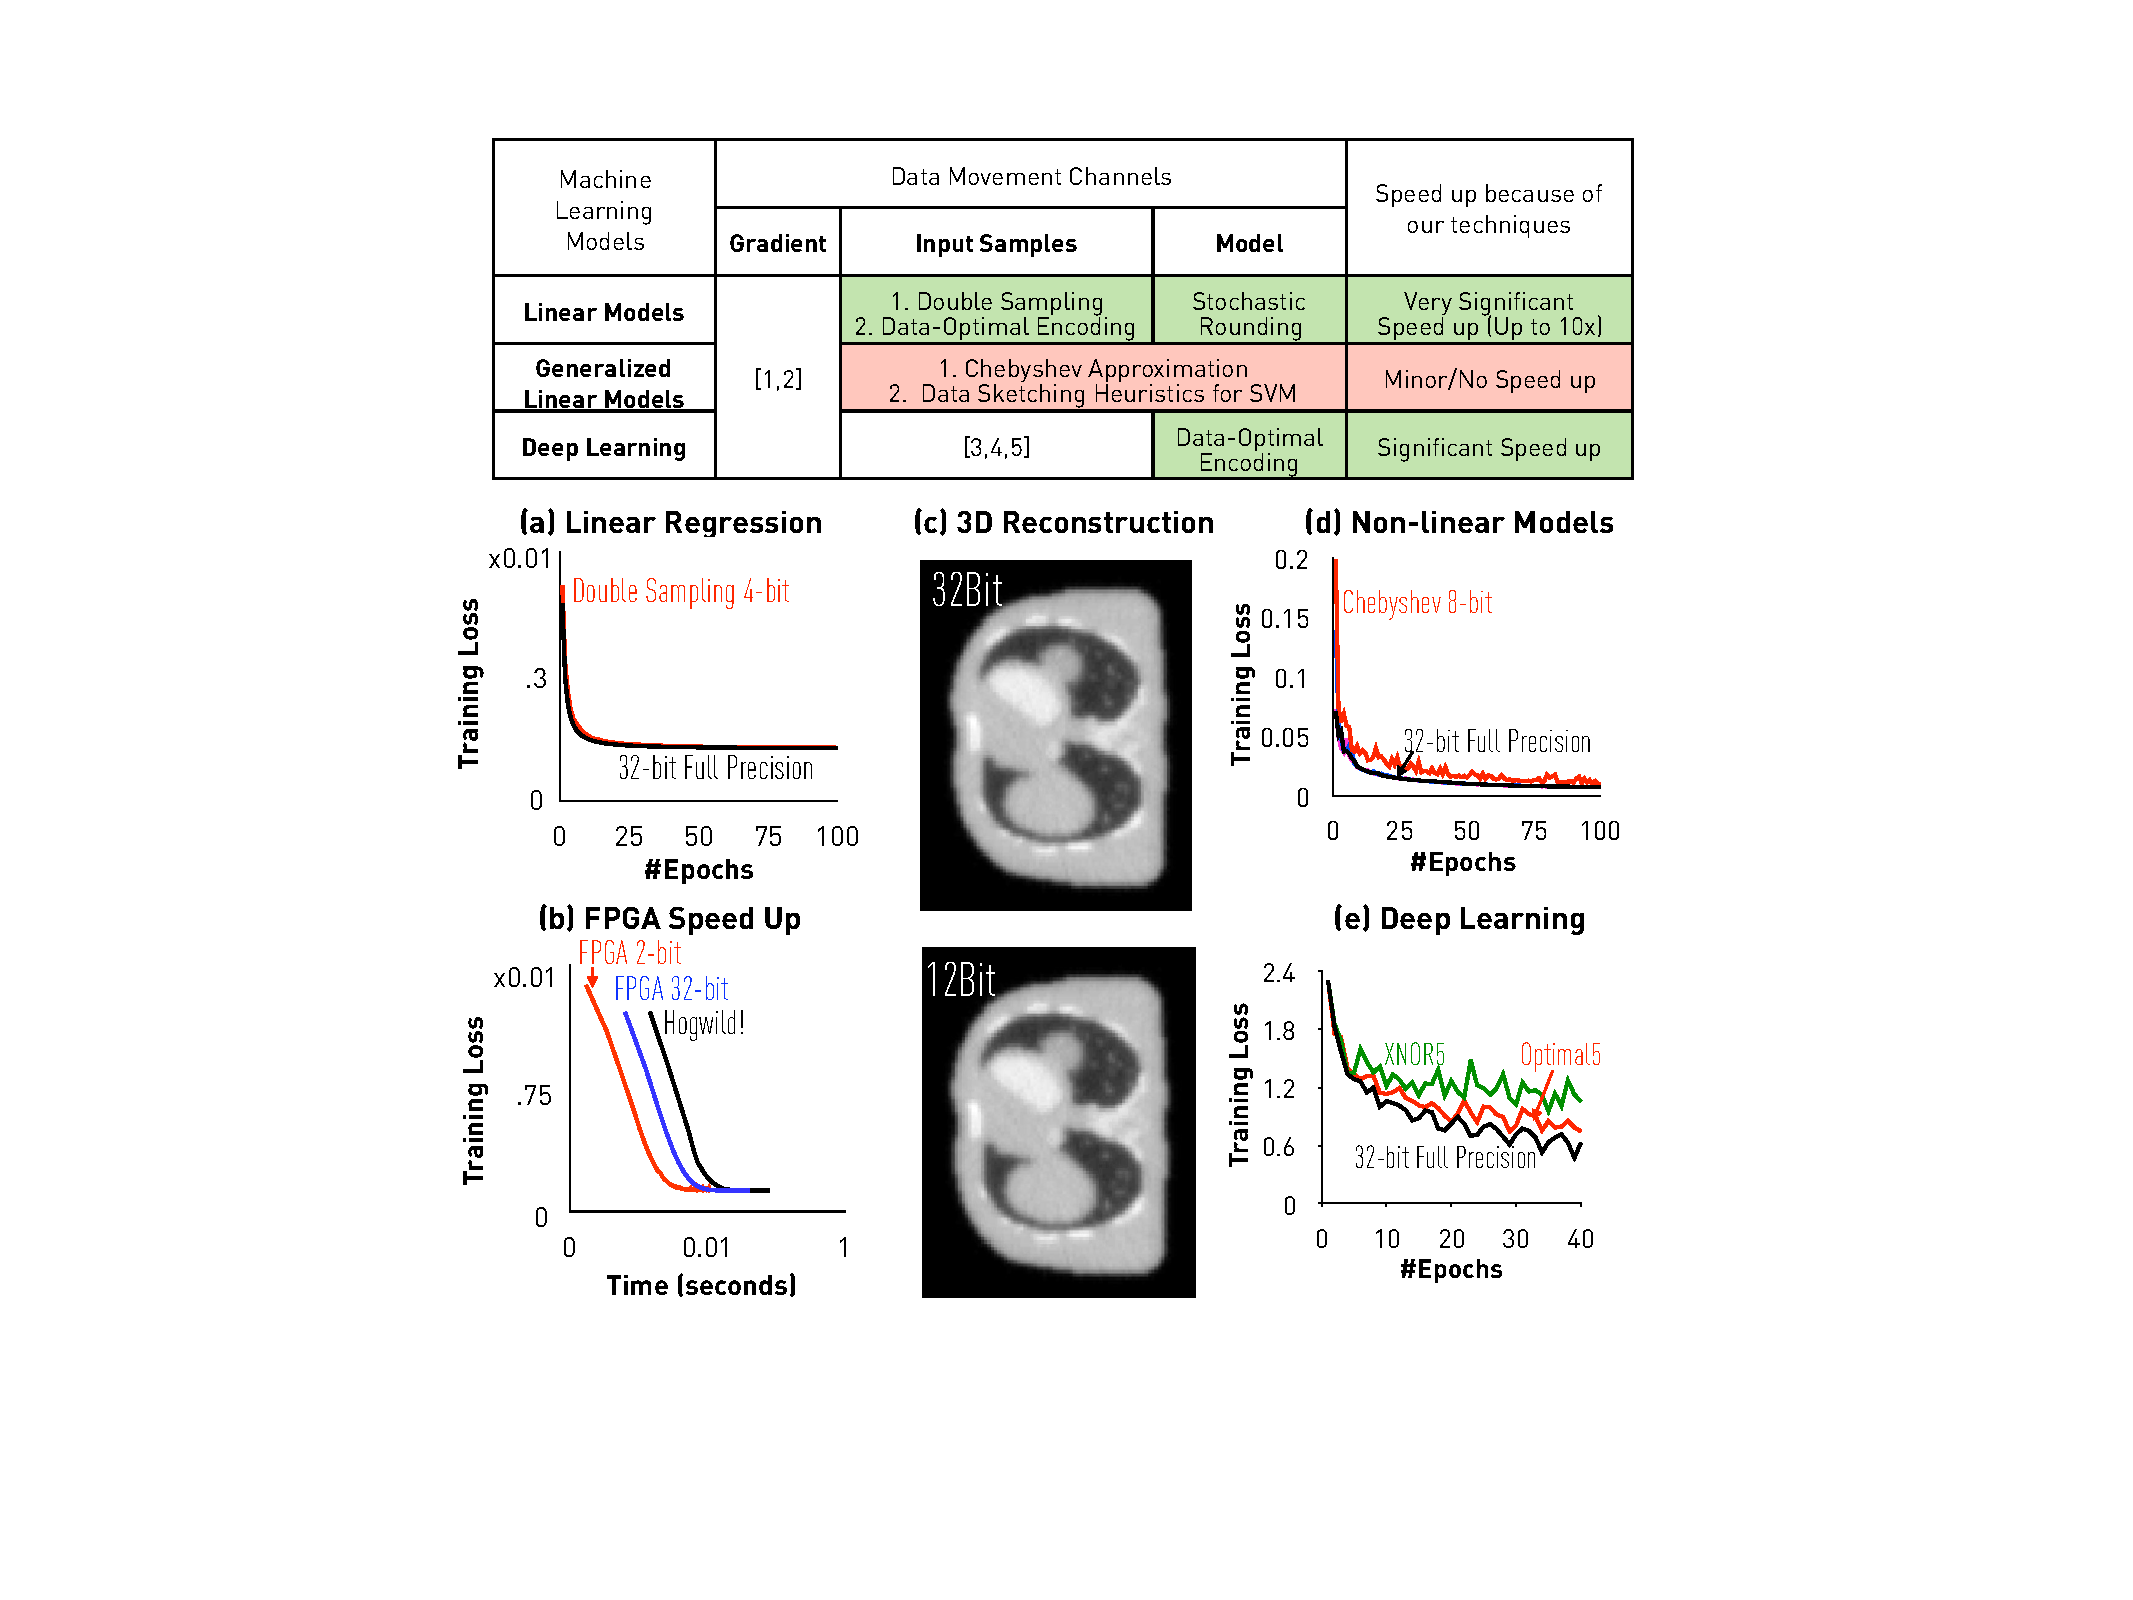
\includegraphics[width=0.5\textwidth]{Figures/RSHighlight}    
\vspace{-2em}
\caption{Overview of theoretical results and
highlights of empirical results. See
Introduction for details.}
\vspace{-1em}
\label{fig:highlight}
\end{figure}

\vspace{-3em}
\section{Introduction}

\vspace{-1em}
The computational cost and power consumption of today's machine learning systems are often driven by data movement, and by the precision of computation. 
In our experience, in applications such as tomographic reconstruction, anomaly detection in mobile sensor networks,
and compressive sensing, the overhead of transmitting the data samples can be massive, 
and hence performance can hinge on reducing the precision of data representation and 
associated computation. 
A similar trend is observed in deep learning, where impressive progress has been reported with systems 
using end-to-end reduced-precision representations~\cite{hubara2016quantized,
rastegari2016xnor,zhou2016dorefa,miyashita2016convolutional}. 
In this context, the motivating question behind our work is:  {\em When training general machine learning models,
can we lower the precision of data representation,
communication, and computation, while maintaining provable guarantees?}
 
In this paper, we develop a general 
framework to answer this question, and
present both positive and negative results
 obtained in the context of this framework. 
 Figure~\ref{fig:highlight} encapsulates our results: 
(a) for linear models, we are able to lower the precision of both computation and communication, including input samples, gradients, and model, by up to $16$ times, while still providing rigorous theoretical guarantees; 
(b) our FPGA implementation of this framework achieves up to $6.5\times$ speedup compared with
a 32-bit FPGA implementation, or with a 10-core CPU running Hogwild!;  
(c) we are able to decrease data movement by $2.7\times$ for
tomographic reconstruction, while obtaining a negligible quality decrease. 
Elements of our framework generalize to (d) non-linear models and (e) model compression for training deep learning models. 
In the following, we describe our technical contributions in more detail. 


\vspace{-1em}
\subsection{Summary of Technical Contributions}
\vspace{-0.5em}

We consider the following problem in training generalized linear models: 
\begin{align}
\min_{\x}:\quad {1\over 2K}\sum_{k=1}^K l(\a_k^\top \x, b_k)^2 + R(\x),
\label{eqn:leastsquares}
\end{align}
where $l(\cdot,\cdot)$ is a loss function and $R$ is a regularization term that could be $\ell_1$ norm, $\ell_2$ norm, or even an indicator function representing the constraint. 
The gradient at the sample $(\a_k, b_k)$ is: 
\[
\g_k := \a_k \frac{\partial l(\a_k^\top \x, b_k)}{\partial \a_k^\top \x} .
\]
We denote the problem dimension by $n$. 
We consider the properties of the algorithm when a lossy compression scheme is applied to the data (samples), 
gradient, and model, to reduce the communication cost of the algorithm---that is, we consider quantization functions $Q_g$, $Q_m$, and $Q_s$ for gradient, model, and samples, respectively, in the gradient update:
\begin{align}
\x_{t + 1} \leftarrow \text{prox}_{\gamma R(\cdot)}\left(\x_t - \gamma Q_g(\g_k (Q_m(\x_t), Q_s(\vec{a}_t)))\right),
\label{eq:proxupdate}
\end{align}
where the proximal operator is defined as
\[
\text{prox}_{\gamma R(\cdot)}(\y) =\argmin_{\x} {1\over 2}\|\x-\y\|^2 + \gamma R(\x).
\]

\vspace{-1.5em}
\paragraph{Our Results} We summarize our results as follows. The {\bf (+)}
sign denotes a ``positive result,'' where we achieve
significant practical speedup; it is {\bf (--)} otherwise.

\vspace{-1em}
\paragraph{(+) Linear Models.} When $l(\cdot,\cdot)$ is 
the least squares loss, we first notice that
simply doing stochastic quantization of data samples  
(i.e., $Q_s$) introduces bias of the gradient
estimator and therefore SGD would converge
to a different solution. We propose a simple
solution to this problem by introducing a
{\em double sampling} strategy
$\tilde{Q}_s$ that uses multiple samples to
eliminate the correlation of samples introduced
by the non-linearity of the gradient. We
analyze the additional variance introduced
by double sampling, and find that its impact is \emph{negligible in terms of convergence time} as long as the 
number of bits used to store a quantized sample is at least $\Theta( \log n / \sigma )$, 
where $\sigma^2$ is the variance of the standard stochastic gradient. 
This implies that the 32-bit precision may be excessive for many practical scenarios. 

\vspace{-0.5em}
We build on this quantization strategy to obtain an \emph{end-to-end quantization} strategy
for linear models that compresses all data movements. 
For certain settings of parameters, end-to-end quantization adds as little as a \emph{constant factor} to the variance of the entire process. 

\vspace{-1.5em}
\paragraph{(+) Optimal Quantization and Extension to Deep Learning.}
We then focus on reducing the variance of  
stochastic quantization. We notice that different methods for setting the quantization points have different variances---the standard uniformly-distributed quantization strategy is far from optimal in many settings.
We formulate this as an independent optimization problem, and solve it optimally with 
an efficient dynamic programming algorithm 
that only needs to scan the data in a single pass.
When applied to linear models, this optimal 
strategy can save up to $1.6\times$ communication
compared with the uniform strategy.

\vspace{-0.5em}
We perform an analysis of the optimal quantizations for various settings, and observe that the uniform quantization approach
popularly used by state-of-the-art end-to-end
low-precision deep learning training systems
when more than 1 bit is used is suboptimal.
We apply optimal quantization to 
model quantization and show that, with one
standard neural network, we outperform the
uniform quantization used by XNOR-Net and a
range of other recent approaches. This
is related, but different, to recent work 
on model compression for inference~\cite{Han:2016:ICLR}. 
To the best of our knowledge, this is the first time such optimal quantization strategies have been applied to training. 

\vspace{-1.5em}
\paragraph{(--) Non-Linear Models.} We extend our
results to non-linear models, such as SVM. We can stretch our multiple-sampling strategy to provide 
unbiased estimators for any polynomials, at the cost of increased variance. 
Building further, we employ Chebyshev polynomials to   
approximate the gradient of \emph{arbitrary smooth loss functions} within arbitrarily low bias, 
and to provide bounds on the error of an SGD solution obtained from low-precision samples. 

Further, we examine whether this approach can be applied to non-smooth loss functions, such as SVM. 
We find that the machinery described above does not apply, for fundamental reasons. 
We use ideas from streaming and dimensionality reduction to develop a variant that is provably correct for non-smooth loss functions. 
We can show that, under reasonable assumptions, the added communication cost of supporting non-smooth functions is negligible. 

\vspace{-0.5em}
In practice, using this technique we are
able to go as low as 8-bit precision for SVM and logistic regression. 
However, we notice that the straw man approach, which applies naive stochastic rounding over the input data to just 8-bit precision, converges to similar results, 
without the added complexity. 
This negative result is explained by the fact that, to approximate non-linearities such as the step function or the sigmoid well, our framework needs both high degree Chebyshev polynomials and relatively large samples. 

\begin{figure}[t]
\centering   
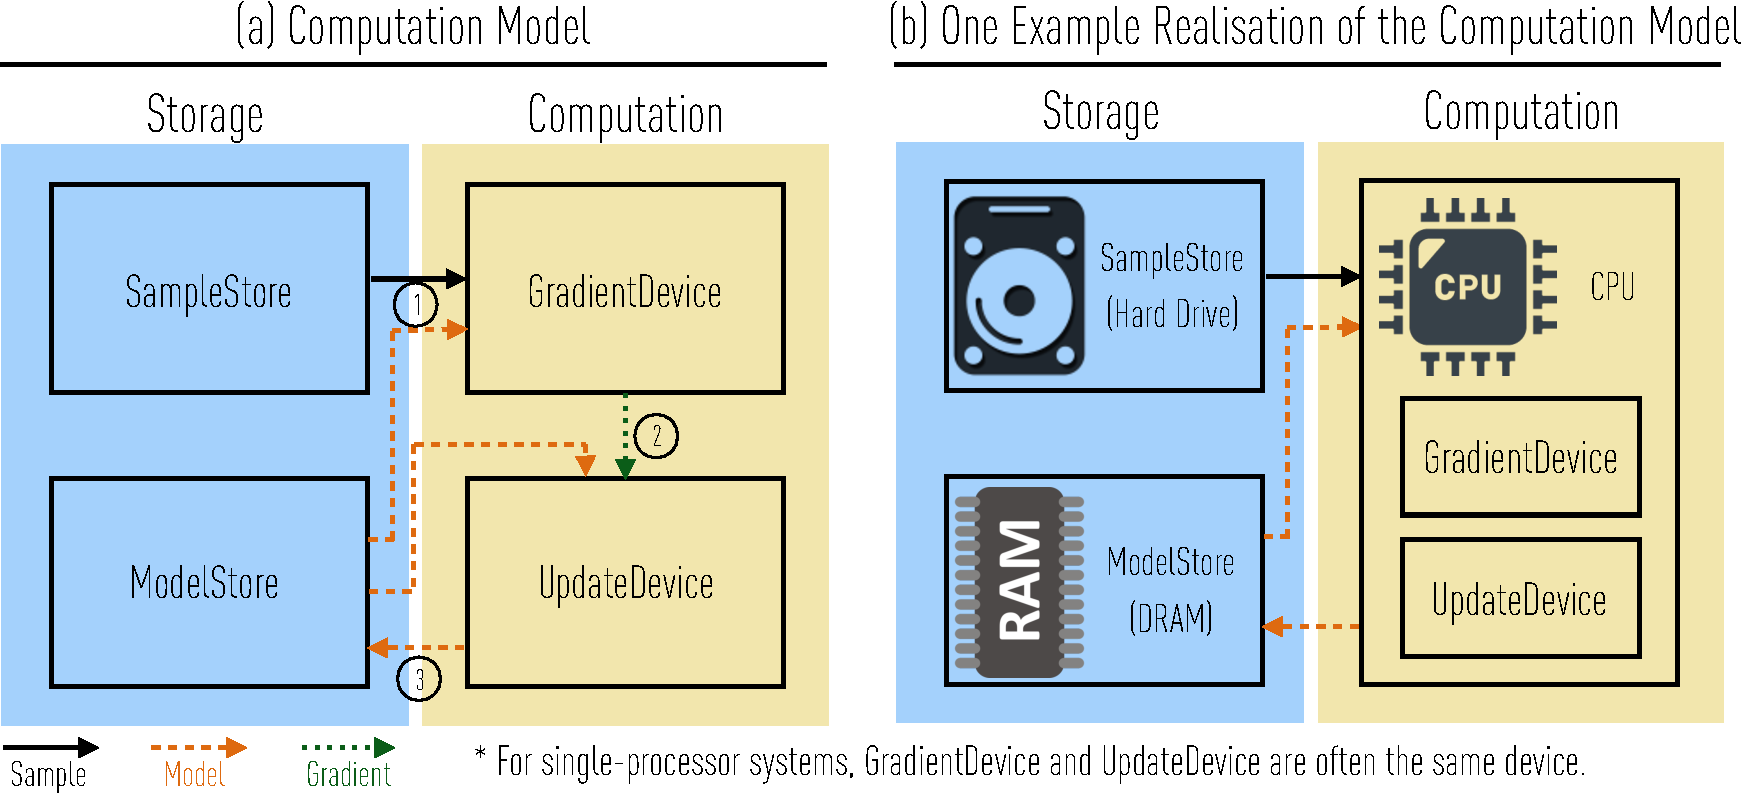
\includegraphics[scale=0.27]{compmodel-pdfcrop}
\vspace{-1em}
\caption{A schematic representation of the computation model.}
\vspace{-0.5em}
\label{fig:model}
\end{figure}


\vspace{-0.5em}
\section{Linear Models}

\vspace{-0.5em}
In this section, we focus on linear models with possibly non-smooth regularization. We have labeled data points $(\a_1, b_1), (\a_2, b_2), \ldots, (\a_K, b_K) \in \R^n \times \R$, and our goal is to minimize the function
\vspace{-0.5em}
\begin{align}
F(\x) = \underbrace{\frac{1}{K} \sum_{k = 1}^K \| \a_k^\top \x - b_k \|_2^2}_{=: f(\x)} + R(\x) \; ,
\label{eq:linear}
\end{align}
i.e., minimize the empirical least squares loss plus a non-smooth regularization $R(\cdot)$ (e.g., $\ell_1$ norm, $\ell_2$ norm, and constraint indicator function). SGD is a popular approach for solving large-scale machine learning problems. It works as follows: at step $\x_t$, given an unbiased gradient estimator $\g_t$, that is, 
$\E(\g_t) = \nabla f(\x_t),$
we update $\x_{t+1}$ by
\[
\x_{t+1} = \text{prox}_{\gamma_t R(\cdot)}\left( \x_t - \gamma_t \g_t\right),
\]
where $\gamma_t$ is the predefined step length. SGD guarantees the following convergence property:
\begin{theorem}\label{thm:sgd-conv}[e.g., \cite{2014arXiv1405.4980B}, Theorem 6.3]
Let the sequence $\{\x_t\}_{t=1}^T$ be bounded. Appropriately choosing the steplength,
we have the following convergence rate for \eqref{eq:linear}:
% 
\begin{equation}
F\left(\frac{1}{T} \sum_{t = 0}^T \x_t\right) - \min_{\x}F(\x) \leq \Theta\left({1\over T} + {\sigma \over \sqrt{T}}\right) 
\label{eq:sgd-conv}
%T = O \left( R^2 \cdot \max \left( \frac{2 \sigma^2}{\epsilon^2} , \frac{L}{\epsilon} \right) \right),
\end{equation}
where $\sigma$ is the upper bound of the mean variance 
\[
\sigma^2 \geq {1\over T}\sum_{t=1}^T \E\|\g_t - \nabla f(\x_t)\|^2. 
\]
%Then $\E \left[ f \left( \frac{1}{T} \sum_{t = 0}^T \x_t \right) \right] - \min_{\x \in \mathcal{X}} f(\x) \leq \epsilon$.
\end{theorem} 
\vspace{-2em}
There are three key factors to ensure for SGD:
\begin{enumerate}
\vspace{-0.75em}
\item Computing stochastic gradient $\g_t$ is cheap;
\vspace{-0.75em}
\item The stochastic gradient $\g_t$ should be unbiased;
\vspace{-0.75em}
\item The stochastic gradient variance $\sigma$ dominates the convergence efficiency, so it needs to be controlled appropriately.
\end{enumerate}
\vspace{-1.5em}
The common choice is to uniformly select one sample:
\vspace{-0.5em}
\begin{align}
\g_t = \g_t^{(full)} := \a_{\pi(t)} (\a_{\pi(t)}^\top \x - b_{\pi(t)}).
\label{eq:sgfull}
\end{align} 
($\pi(t)$ is a uniformly random integer from $1$ to $K$). We abuse the notation and let $\a_t = \a_{\pi(t)}$. Note that $\g_t^{(full)}$ is an unbiased estimator $\E [\g_t^{(full)}] = \nabla f(\x_t)$. Although it has received success in many applications, 
if the precision of sample $\a_{t}$ can be further decreased,
we can save potentially one order of magnitude bandwidth
of reading $\a_{t}$ (e.g., in sensor networks) and the associated computation (e.g.,
each register can hold more numbers). 
This motivates us to use low-precision sample points to train the model. The following will introduce the proposed low-precision SGD framework by meeting all three factors for SGD.

\vspace{-0.5em}
\subsection{Stochastic Quantization for Saving Bandwidth} 
\vspace{-0.5em}

We propose to use stochastic quantization to generate a low-precision version of an arbitrary vector $\v$ in the following 
way. Given a vector
$\v$, let $M(\v)$ be a scaling factor such that $-1 \le \v/M(\v) \le 1$. Without loss of generality, let $M(\v)=||\v||_2$. We partition the interval $[-1, 1]$ using $s+1$ separators: $-1 = l_0 \le l_1 ... \le l_{s} = 1$; for each number $v$ in $\v/M(\v)$, we 
quantize it to one of two nearest separators: $l_i \le v \le l_{i+1}$. We denote the \emph{stochastic quantization} function by $Q(\v, s)$ and choose the probability of quantizing to different separators such that $\E[Q(\v, s)] = \v$. We use $Q(\v)$ when $s$ is not relevant.

\vspace{-0.5em}
\subsection{Double Sampling for Unbiased Stochastic Gradient}
\vspace{-0.5em}

\begin{wrapfigure}{r}{0.23\textwidth}
  \begin{center}
    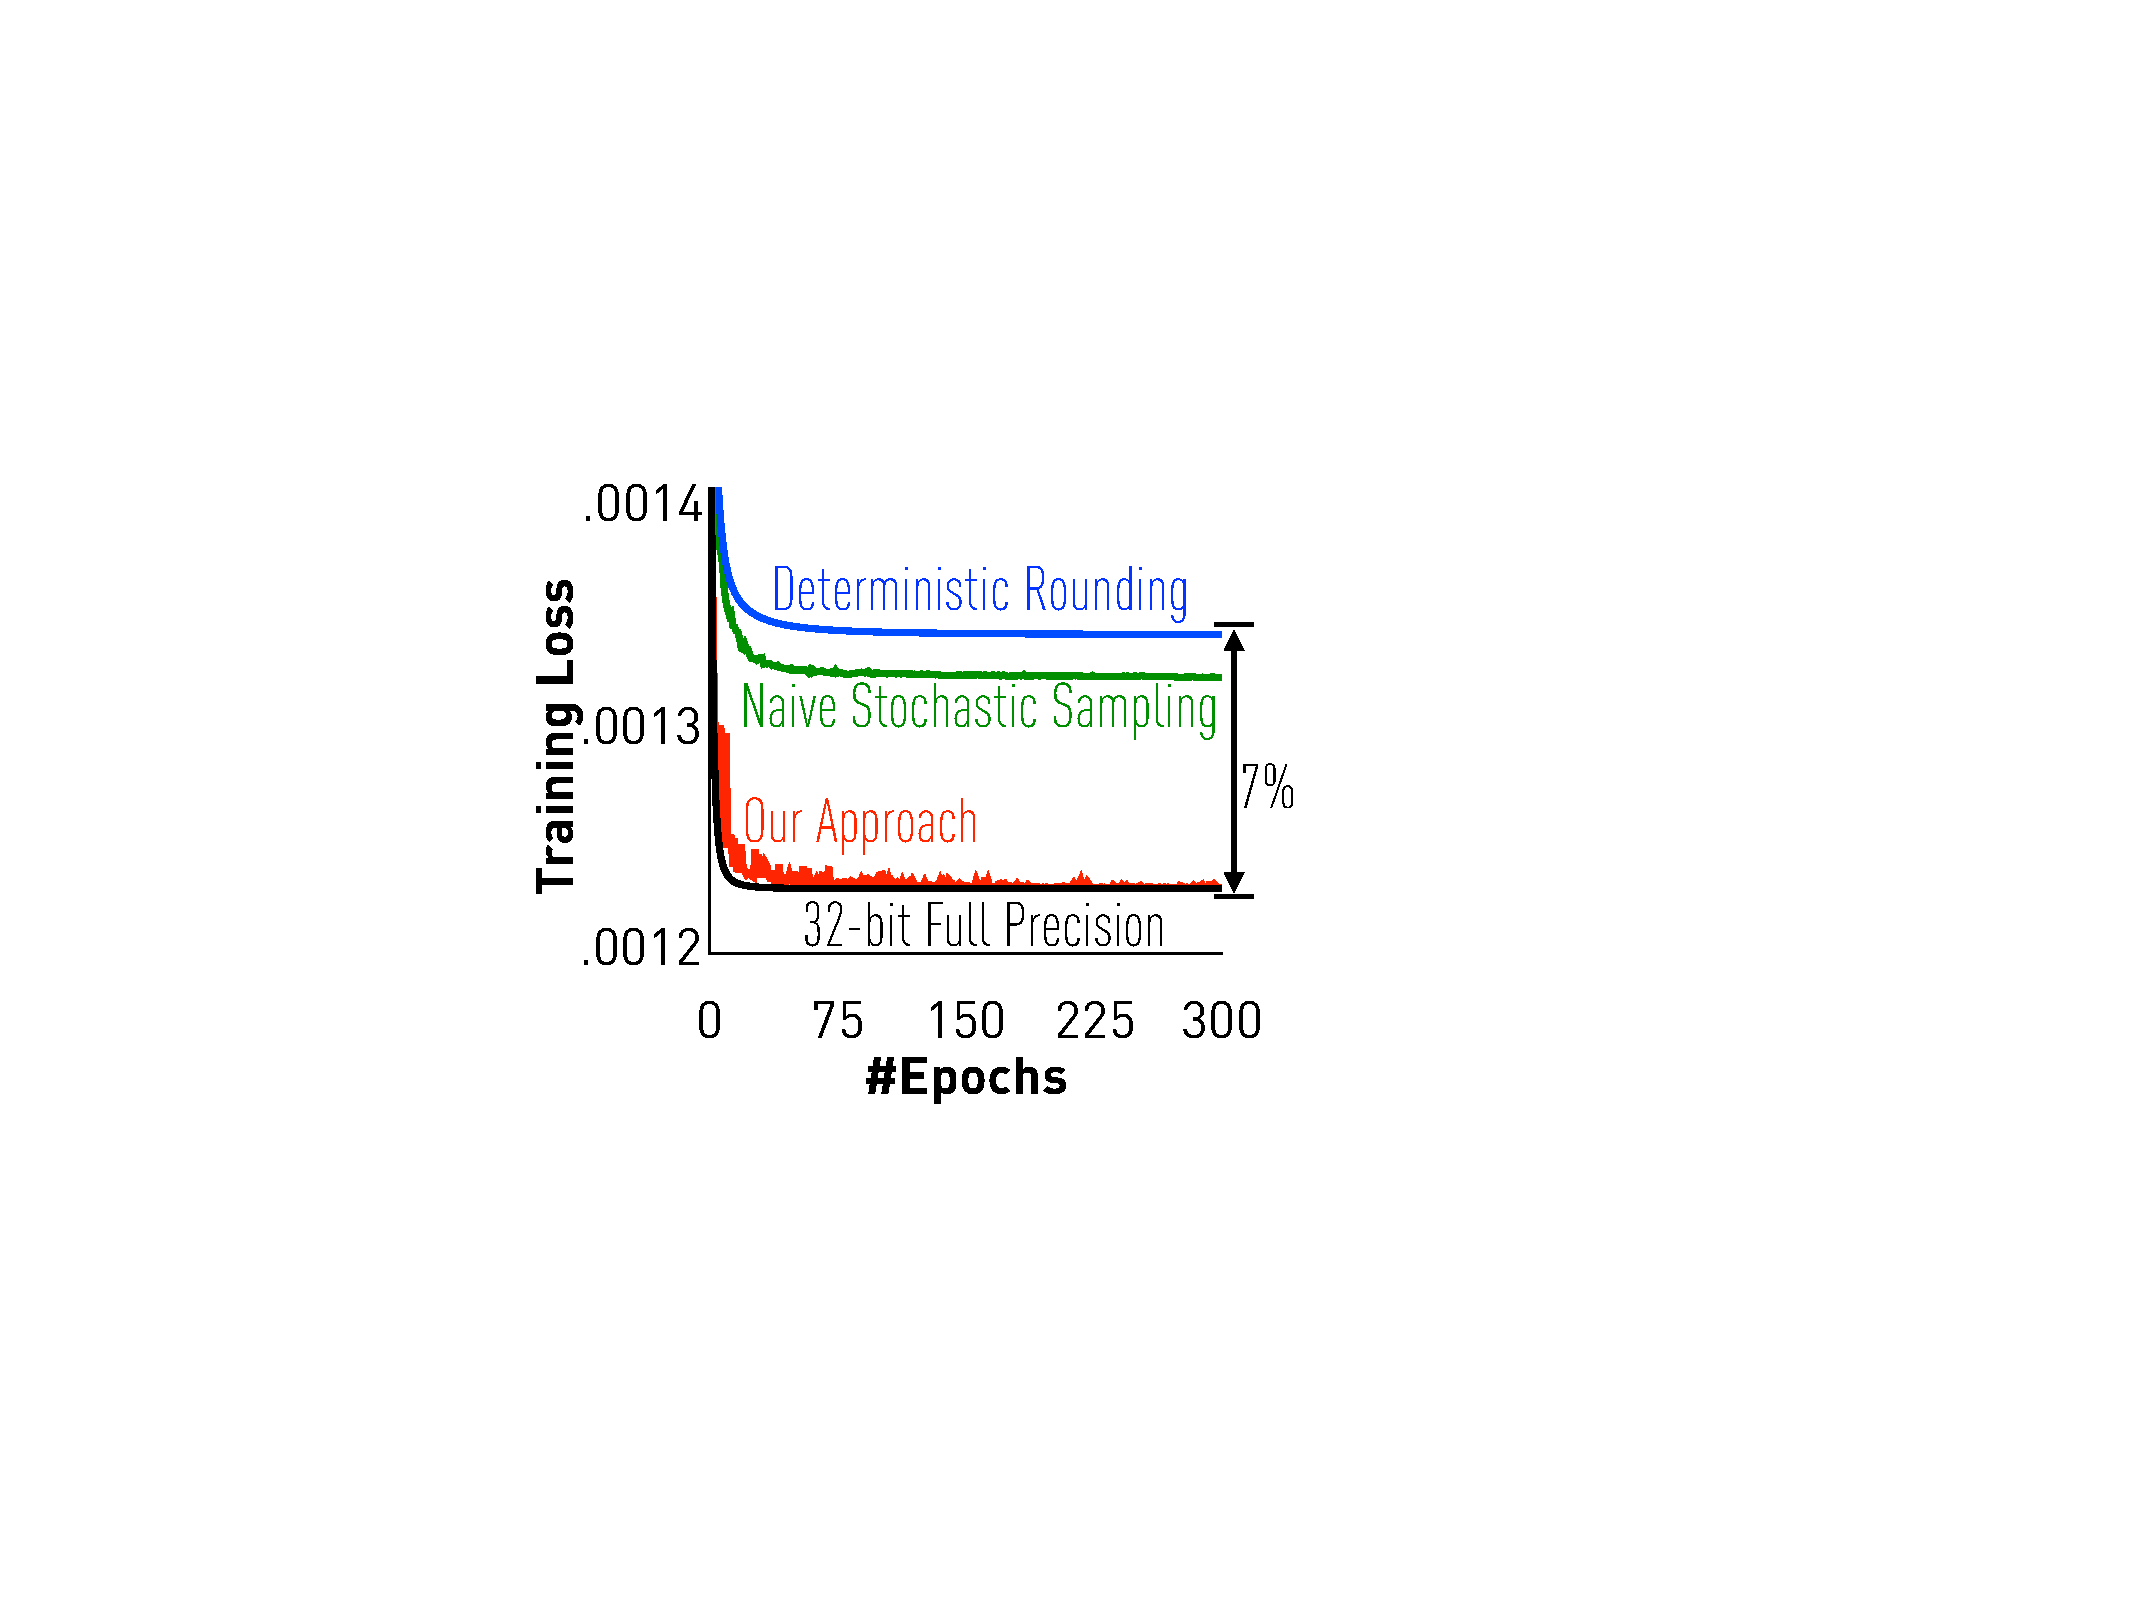
\includegraphics[width=0.23\textwidth]{micro-experiments/gap.pdf}
  \end{center}
  \label{fig:gap}
\end{wrapfigure}
The naive way to use low-precision samples $\hat{\a}_t := Q(\a_t)$ is 
\[
\hat{\g}_t := \hat{\a}_t \hat{\a}_t^\top \x - \hat{\a}_t b_t.
\]
However, \emph{the naive approach does not work} (that is, it does not guarantee convergence), because it is biased: 
\[
\E[\hat{\g}_t] := \a_t \a_t^\top \x - \a_t b_t + D_{\a} \x, 
\]
where $D_{\a}$ is diagonal and its $i$th diagonal element is 
\[
\E[ Q(\a_i)^2 ] - \a_i^2.
\]

\vspace{-0.5em}
Since $D_{\a}$ is non-zero, we obtain a \emph{biased} estimator of the gradient, so the iteration is unlikely to converge. 
The figure on the right illustrates the bias caused by a non-zero $D_{\a}$. In fact, it is easy to see that in instances where the minimizer $\x$ is large and gradients become small, we will simply diverge. 

We now present a simple method to fix the biased gradient estimator. We generate two independent random quantizations and revise the gradient:
\begin{align}
\g_t := Q_1 (\a_t) (Q_2 (\a_t)^\top \x + b_t) \; .
\label{eq:double}
\end{align}
This gives us an unbiased estimator of the gradient. 

\paragraph*{Overhead of Storing Two Samples}
The reader may have noticed that one implication of double sampling is the overhead of sending
two samples instead of one. We note that this will not introduce $2\times$
overhead in terms of data communication. Instead, just one additional bit
is needed for the second sample because of correlation, as the two samples 
differ by at most one bit. More generally, since samples
are used symmetrically, sending $k$ samples only requires $\log_2 k$ more bits.

\vspace{-0.5em}
\subsection{Variance Reduction}
\vspace{-0.5em}

From Theorem~\ref{thm:sgd-conv}, the mean variance ${1\over T}\sum_{t}\E\|\g_t - \nabla f(\x)\|^2$ will dominate the convergence efficiency. It is not hard to see that the variance of the double sampling based stochastic gradient in \eqref{eq:double} can be decomposed into
\vspace{-0.5em}
\begin{align*}
\E\|\g_t - \nabla f(\x_t)\|^2 & \leq \E \|\g_t^{(full)}- \nabla f(\x_t)\|^2 
\\
&+ \E \|\g_t - \g_t^{(full)})\|^2.
\end{align*}
The first term is from the full stochastic gradient, which can be reduced by using strategies such as mini-batch, weight sampling, and so on. Reducing the first term is issue orthogonal to this paper. 
Rather, we are interested in the second term, which is the additional cost of using low-precision samples. All strategies for reducing the variance of the first term can seamlessly combine with the approach of this paper. 
The additional cost can be bounded by the following lemma.
\begin{lemma} 
The stochastic gradient variance using double sampling in \eqref{eq:double} $\E\|\g_t - \g_t^{(full)}\|^2$ can be bounded by
\begin{align*}
%&\E\|\g_t - \g_t^{(full)}\|^2 \leq \\
&\Theta\left(\mathcal{TV}(\a_t) (\mathcal{TV}(\a_t)\|\x\odot \x\| + \|\a_t^\top \x\|^2 + \|\x\odot \x\|\|\a_t\|^2)\right),
\end{align*}
where $\mathcal{TV}(\a_t) := \E\|Q(\a_t) - \a_t\|^2$ and $\odot$ denotes the element product.
\end{lemma}
Thus, minimizing $\mathcal{TV}(\a_t)$ is key to reducing variance. 

\vspace{-0.5em}
\paragraph{Uniform quantization} It makes intuitive sense that, the more levels of quantization, the lower the variance. The following result shows the quantitative dependence between the variance and the number of uniformly distributed levels. 

\begin{lemma}
\label{lem:quant-facts} [\cite{Alistarh:2016:ArXiv}]
Assume that quantization levels are uniformly distributed. For any vector $\vec{v} \in \R^n$, we have that $\E [Q (\vec{v},s)] = \vec{v}$; furthermore, the total variance using uniform quantization with level $s$ is bounded by
\[
\mathcal{TV}_s(\v):=\E [\| Q (\vec{v},s) - \v\|_2^2] \leq \min( n/s^2,\sqrt{n}/s)) \| \vec{v} \|_2^2. \; .
\]
\end{lemma} 

\vspace{-1em}
Together with other results, it suggests the stochastic gradient variance of using double sampling is bounded by
\[
\E\|\g_t - \nabla f(\x_t)\|^2 \leq \sigma^2_{(full)} + \Theta \left( {n /s^2} \right),
\]
where $\sigma^2_{(full)} \geq \E \|\g_t^{(full)} - \nabla f(\x)\|^2$ is the upper bound of using the full stochastic gradient, assuming that $\x$ and all $\a_k$'s are bounded. Because the quantization level $s$ is exponential to the number of bits, to ensure that these two terms are comparable (using a low-precision sample does not degrade the convergence rate), the number of bits only needs to be greater than $\Theta (\log n /\sigma_{(full)})$. Even for linear models with millions
of features, 32 bits is likely to be  ``overkill.''

\vspace{-0.5em}
The uniform quantization provides us an intuitive dependence between variance and the level of quantization. However, in practice, we can do better by designing the optimal quantization separation given the quantization level $s$. This motivates
our study in the next section.





\vspace{-1em}
\section{Optimal Quantization Strategy for Reducing Variance} \label{sec:optimal}

\vspace{-0.5em}

In the previous section, we have assumed uniformly distributed quantization points.  
We now investigate the choice of quantization points and present an optimal strategy to minimize the quantization variance term $\mathcal{TV}(\a_t)$.

\vspace{-1em}
\paragraph*{Problem Setting}
Assume a set of real numbers $\Omega = \{x_1, \ldots, x_N\}$ with cardinality $N$. WLOG, assume that all numbers are in $[0, 1]$ and are sorted such that $x_1 \leq \ldots \leq x_N$. 

The goal is to partition $\setI = \{I_j\}_{j = 1}^s$ of $[0, 1]$ into $s$ disjoint intervals, so that if we randomly quantize every $x \in I_j$ to an endpoint of $I_j$, the variance is minimal over all possible partitions of $[0, 1]$ into $k$ intervals.
Formally:
\vspace{-0.5em}
\begin{align}
\nonumber \min_{\setI: |\setI| = s} \quad & \mathcal{MV}(\setI) := {1\over N}\sum_{j = 1}^k \sum_{x_i \in I_j} \err(x_i, I_j)\\
\text{s.t.}\quad & \bigcup_{j = 1}^s I_j = [0, 1],\quad I_j\cap l_k = \emptyset~\text{for $k\neq j$},
\label{eq:opt_Q}
\end{align}
where $\err (x, I) = (b - x) (x - a)$ is the variance for point $x \in I$ if we quantize $x$ to an endpoint of $I = [a, b]$.
That is, $\err (x, I)$ is the variance of the (unique) distribution $D$ supported on ${a, b}$ so that $\E_{X \sim D} [X] = x$.

Given an interval $I \subseteq [0, 1]$, we let $\setX_I$ be the set of $x_j \in \setX$ contained in $I$.
We also define $\err (\setX, I) = \sum_{x_j \in I} \err (x_j, I)$.
Given a partition $\setI$ of $[0, 1]$, we let $\err (\setX, \setI) = \sum_{I \in \setI} \err (\setX, I)$.
We let the optimum solution be $\setI^* = \argmin_{|\setI| = k} \err (\setX, \setI)$, breaking ties randomly. 

\vspace{-1em}
\subsection{Dynamic Programming}
\vspace{-0.5em}

We first present a dynamic programming algorithm that solves the above problem in an exact way. In the next subsection, we present a more practical approximation algorithm that only needs to scan all data points \emph{once}.

\vspace{-0.5em}
One challenge is due to non-convexity and non-smoothness. 
We start from the observation that there exists an optimal solution that places endpoints at input points. 

\begin{lemma}
\label{lem:discrete}
There is a $\setI^*$ so that all endpoints of any $I \in \setI^*$ are in $\Omega \cup \{0, 1\}$.
\end{lemma}


\iffalse
\begin{proof}
Fix any endpoint $b$ of intervals in $\setI^*$. WLOG assumes that $b \neq 0, 1$. Then we must have $I = [a, b]$ and $I' = [b, c]$ for some $I, I' \in \setI^*$. Observe that the choice of $b$ only affects the error for points in $I \cup I'$. We have that $\err (\Omega, I) + \err (\Omega, I') $ is given by 
\begin{align*}
& \sum_{x \in I} (b - x) (x - a) + \sum_{x \in I'} (c -x)(x - b) \\
&= A b + C \; ,
\end{align*}
where $A, C$ are constants that do not depend on $b$. Hence, this is a linear objective in $b$. Since $b$ can freely range between the rightmost point in $I$ and the leftmost point in $I'$, there is an optimizer for this solution at one of those two points. Hence we may choose $b \in \Omega$.
\end{proof}
\fi

\vspace{-0.5em}
Therefore, to solve the problem in an exact way, we just need to select a subset of data points in $\Omega$ as quantization points. Define $T(k, m)$ be the optimal total variance for points in $[0, d_m]$ with $k$ quantization levels choosing $d_m=x_m$ for all $m=1,2,\cdots, N$. Our goal is to calculate $T(s, N)$. This problem can be solved by dynamic programing using the following recursion
\[
T(k, m) = \min_{j\in \{k-1, k, \cdots, m-1\}} T(k-1,j) + V(j,m),
\]
where $V(j,m)$ denotes the total variance of points falling into $[d_j, d_m]$. The complexity of calculating the matrix $V(\cdot, \cdot)$ is $O(N^2 + N)$ and the complexity of calculating matrix $T(\cdot, \cdot)$ is $O(kN^2)$. The memory cost is $O(kN + N^2)$. 

\begin{figure}[t]
\centering    
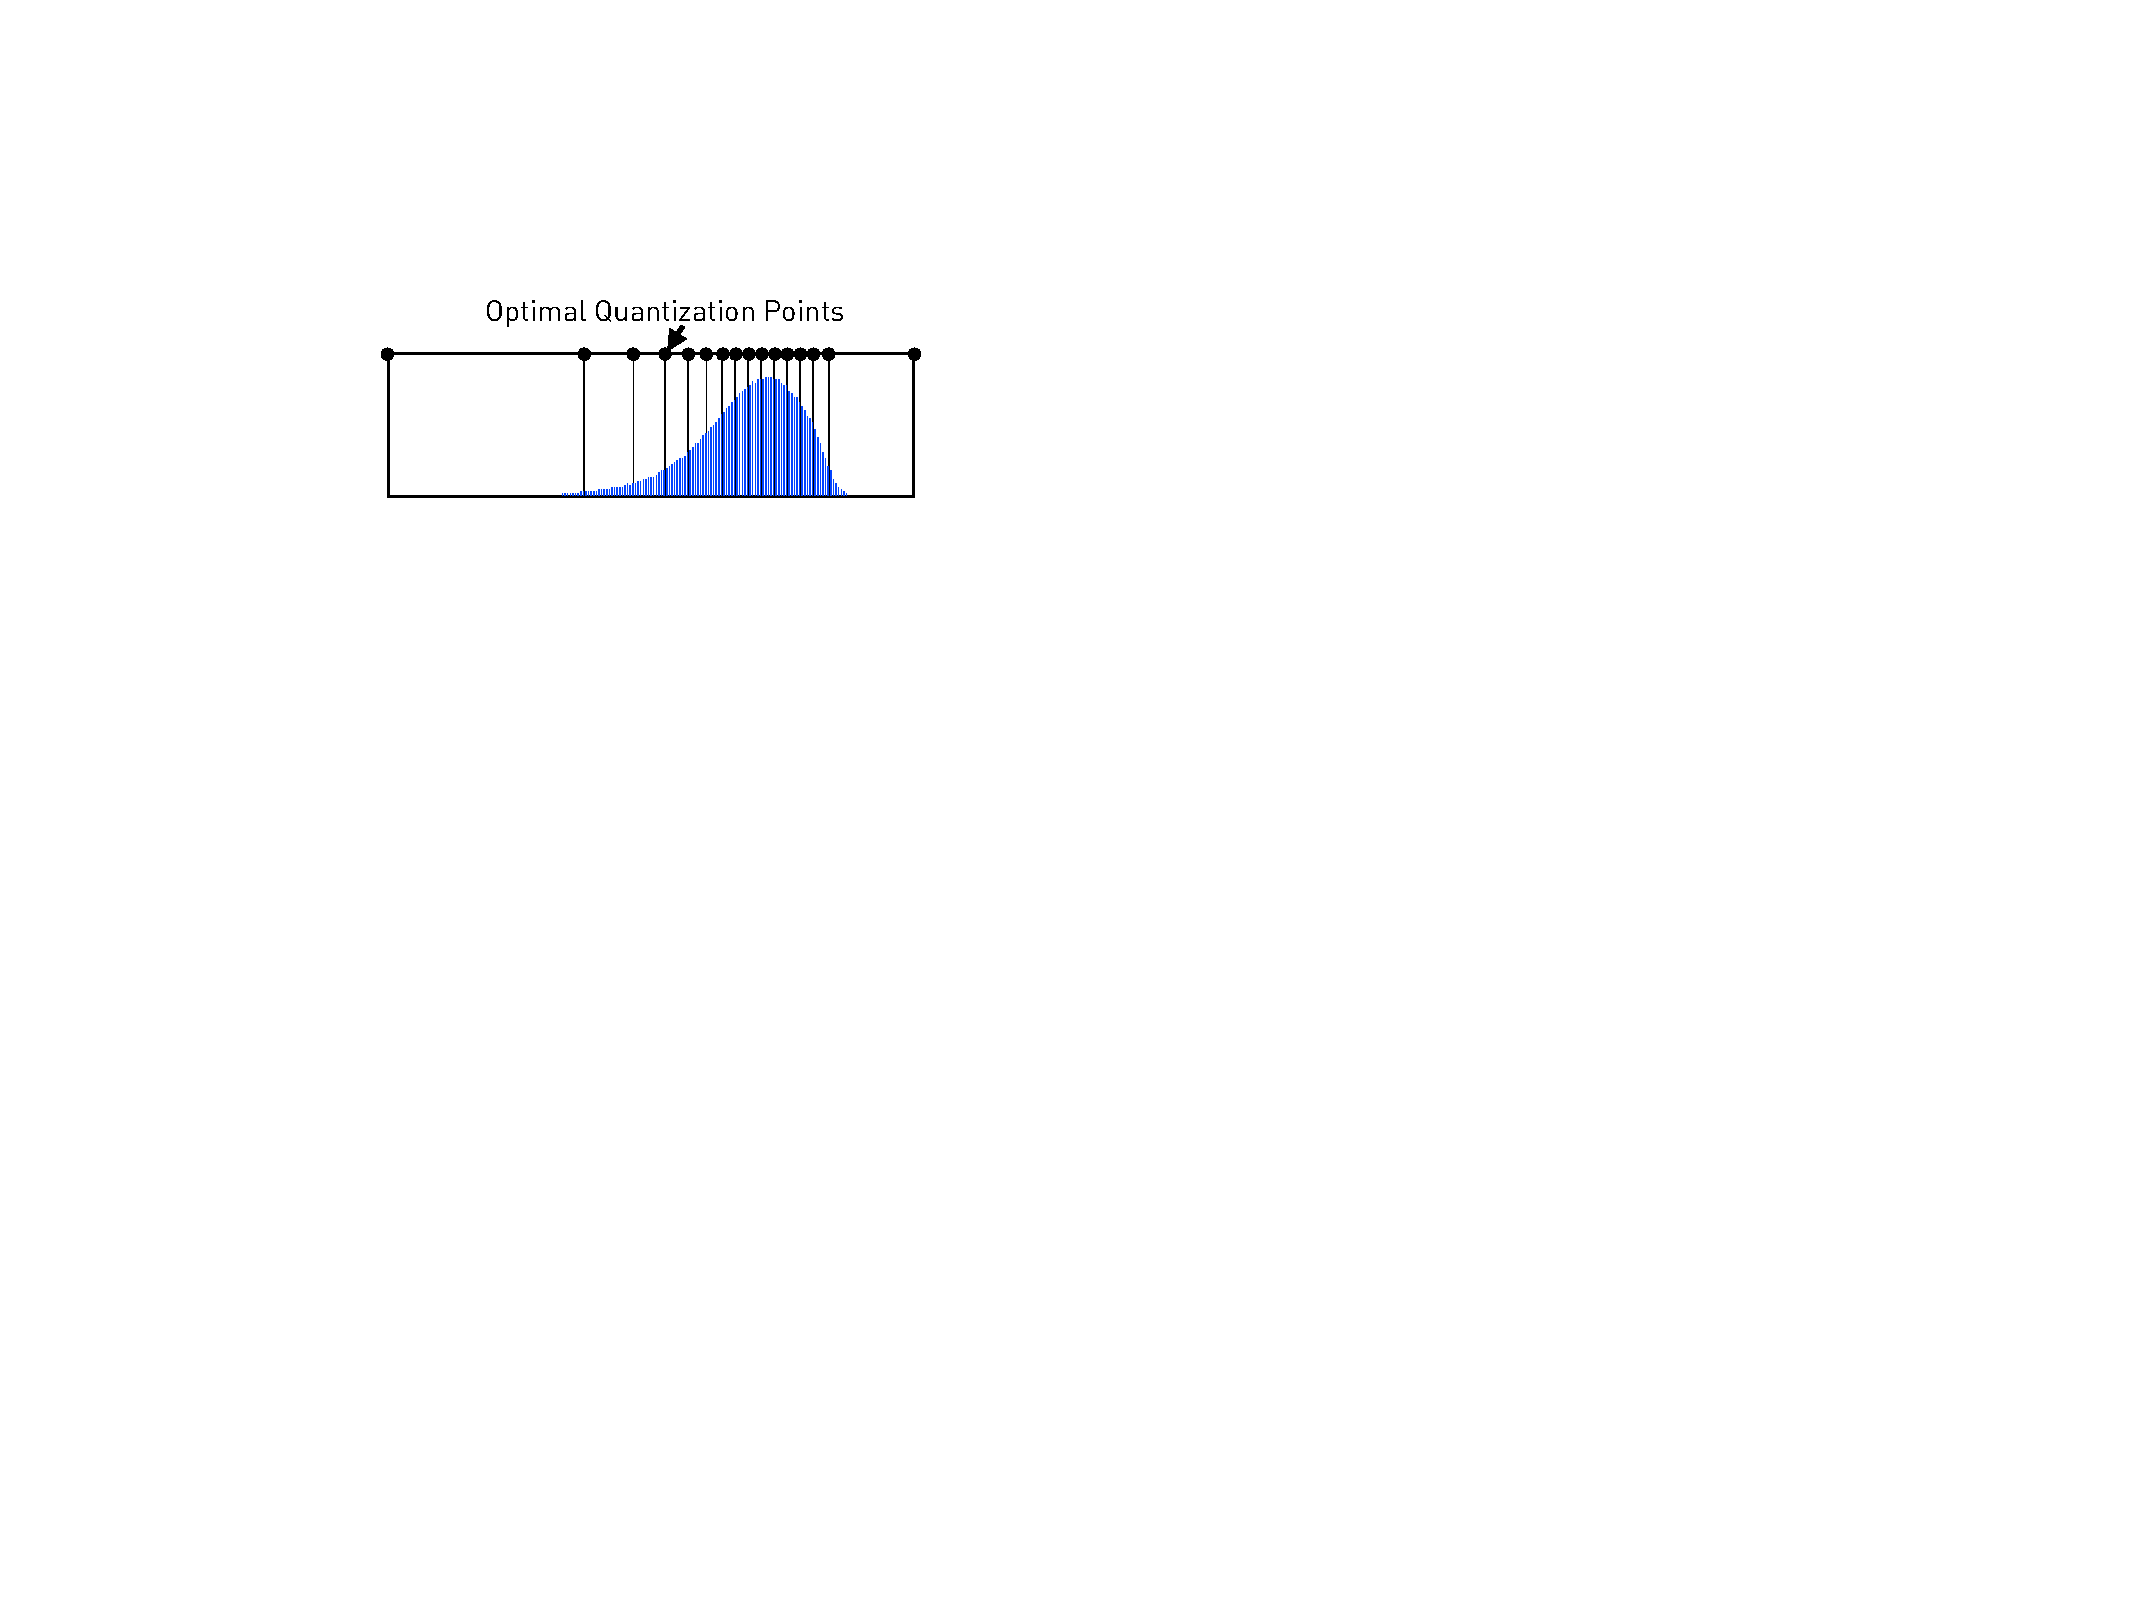
\includegraphics[width=0.5\columnwidth]{micro-experiments/dp-level.pdf} 
\vspace{-1em}
\caption{Optimal quantization points calculated with
dynamic programming given a data distribution. }
\vspace{-1em}
\label{fig:optimalquantization}
\end{figure} 

\vspace{-0.5em}
\subsection{Heuristics}
\vspace{-0.5em}

The exact algorithm has a complexity that is quadratic to the number of data points. To make our algorithm practical,
we develop an approximation algorithm that only needs to scan all data points once and has linear complexity to $N$.

\vspace{-0.5em}
\paragraph*{Discretization}

We can discretize the range $[0,1]$ into $M$ intervals, i.e., $[0,d_1), [d_1, d_2), \cdots, [d_{M-1}, 1]$ with $0< d_1<d_2<\cdots < d_{M-1}<1$. We then restrict our algorithms to only choose $k$ quantization points within these $M$ points, instead of all $N$ points in the exact algorithm. The following result bounded the quality of this approximation.

\begin{theorem} \label{thm:optQ}
Let the maximal number of data points in each ``small interval'' (defined by $\{d_m\}_{m=1}^{M-1}$) and the maximal length of small intervals be bounded by $bN/M$ and $a/M$, respectively. Let ${\mathcal{I}^*} := \{l^*_j\}_{k=1}^{k-1}$ and $\hat{\mathcal{I}}^* :=\{\hat{l}^*_k\}_{k=1}^{k-1}$ be the optimal quantization to \eqref{eq:opt_Q} and the solution with discretization. Let $cM/k$ be the upper bound of the number of small intervals crossed by any ``large interval'' (defined by ${\mathcal{I}}^*$). Then we have the discretization error bounded by
\vspace{-0.5em}
\[
 \mathcal{MV}(\hat{\mathcal{I}}^*) -  \mathcal{MV}({\mathcal{I}}^*) \leq {a^2b k \over 4 M^3} + {a^2bc^2 \over Mk}.
\]
\end{theorem}

\vspace{-0.5em}
Theorem~\ref{thm:optQ} suggests that the mean variance using the discrete variance-optimal quantization will converge to the optimal with the rate $O(1/Mk)$.

\vspace{-0.5em}
\paragraph*{Dynamic Programming with Candidate Points}
Notice that we can apply the same dynamic programming approach given $M$ candidate points. 
In this case, the total computational complexity becomes $O((k+1)M^2 + N)$, with memory cost 
$O(kM + M^2)$. Also, to find the optimal quantization,  we only need to scan all $N$ numbers once.
Figure~\ref{fig:optimalquantization} illustrates an example output for our algorithm.

\vspace{-0.5em}
\paragraph*{$2$-Approximation in Almost-Linear Time} 
In the supplementary material, we present an algorithm which, given $\Omega$ and $k$, provides a split using at most $4 k$ intervals, which guarantees a $2$-approximation of the optimal variance for $k$ intervals, using $O( N \log N )$ time. This 
is a new variant of that by (Acharya et al., 2015) for the histogram recovery problem. 
We can use the $4k$ intervals given by this algorithm as candidates for the DP solution, to get a general $2$-approximation using $k$ intervals in time $O( N \log N + k^3)$. 

\vspace{-1.0em}
\subsection{Extension to Deep Learning}
\vspace{-0.5em}

In this section, we show that it is possible 
to apply optimal quantization to
training deep neural networks.

\vspace{-0.5em}
\paragraph*{State-of-the-art} We focus on
training deep neural networks with a quantized
model. Let $\mathcal{W}$ be the model and 
$l(\mathcal{W})$ be the loss function. State-of-the-art quantized networks,
such as XNOR-Net and QNN, replace $\mathcal{W}$
with the quantized version $Q(\mathcal{W})$, and optimize
for
\[
\min_{\mathcal{W}} l(Q(\mathcal{W})).
\]
With a properly defined 
$\frac{\partial Q}{\partial{\mathcal{W}}}$, we can
apply the standard backprop 
algorithm.
Choosing the quantization function $Q$ is
an important design decision. For 1-bit quantization,
XNOR-Net searches the optimal quantization point. However, for multiple bits,
XNOR-Net, as well as other approaches such as QNN, resort
to uniform quantization.

\vspace{-1.0em}
\paragraph*{Optimal Model Quantization for Deep Learning}

We can apply our optimal quantization strategy 
and use it as the quantization function $Q$
in XNOR-Net. Empirically, this results in 
quality improvement
over the default {\em multi-bits} quantizer in XNOR-Net. 
In spirit, our approach is similar to the 1-bit quantizer of
XNOR-Net, which is equivalent to our approach when the data
distribution is symmetric---we extend this
to multiple bits in a principled way. Another related work
is the uniform quantization strategy 
in {\em log domain}~\cite{miyashita2016convolutional},
which is similar to our approach when the data distribution
is ``log uniform.'' However, our approach does not rely on
any specific assumption of the data distribution.
\citet{Han:2016:ICLR} use $k$-means to
compress the model for {\em inference}~---$k$-means
optimizes for a similar, but different, objective
function than ours. In this paper, we 
develop a dynamic
programming algorithm to do optimal stochastic quantization efficiently.



\vspace{-1em}
\section{Non-Linear Models}
\vspace{-0.5em}

In this section, we extend our framework to approximate arbitrary classification losses within arbitrarily small bias. 

\vspace{-0.5em}
\subsection{Quantizing Polynomials} 
\vspace{-0.5em}

Given a degree $d$ polynomial $P(x) = \sum_{i = 0}^{d} m_i z^i$,
our goal is to evaluate at $\vec{a}^\top \vec{x}$, while quantizing $\vec{a}$, so as to preserve the value of $P( \vec{a}^\top \vec{x})$ in expectation. 

\vspace{-0.5em}
We will use $d$ independent quantizations of $\vec{a}$, $Q_1(\vec{a}), Q_2(\vec{a}), \ldots, Q_d(\vec{a})$. 
Given these quantizations, our reconstruction of the polynomial at $( \vec{a}^\top \vec{x})$ will be 
\vspace{-0.5em}
$$ Q(P) := \sum_{i = 0}^d m_i \prod_{j \leq i} Q_j(\vec{a})^\top \vec{x}.$$

\vspace{-1em}
The fact that this is an unbiased estimator of $P( \vec{a}^\top \vec{x} )$ follows from the independence of the quantizations. Using Lemma~\ref{lem:quant-facts} yields:

\vspace{-0.5em}
\begin{lemma}
\label{lem:poly-sec-moment-bound}
	$\E[ Q(P)^2 ] \leq \left(\sum_{i = 0}^d m_i r(s)^i (\vec{a}^\top \vec{x})^i\right)^2.$
\end{lemma} 
\vspace{-0.5em}


\vspace{-0.5em}
\subsection{Quantizing Smooth Classification Losses}
\vspace{-0.5em}

We now examine a standard classification setting, where samples $[(\vec{a}_i, b_i)]_i$ are drawn from a distribution $\mathcal{D}$. Given a smooth loss function $\ell: \R \rightarrow \R$, we wish to find $\vec{x}$ which minimizes $\E_{\mathcal{D}} [ \ell( b \cdot \vec{a}^\top \vec{x}) ]$. The gradient of $\ell$ is given by 
$$ \nabla_\vec{x} (b \cdot \vec{a}^\top \vec{x}) = b \ell' (b \cdot \vec{a}^\top \vec{x}) \vec{a}.$$

Assume normalized samples, i.e. $\| \vec{a}_i \|_2 \leq 1, \forall i$, and that $\vec{x}$ is constrained such that $\| \vec{x} \|_2 \leq R$, for some real value $R > 0$. We wish to approximate the gradient within some target accuracy $\epsilon$. 

\vspace{-0.5em}
To achieve this, fix a minimal-degree polynomial $P$ such that $|P(z) - \ell'(z)| \leq \epsilon, \forall z \leq R$. Assume this polynomial is known to both transmitter (sample source) and receiver (computing device). The protocol is as follows. 
\vspace{-0.5em}
\begin{itemize}
    \vspace{-0.5em}
	\item For a given sample $(\vec{a}_i, b_i)$ to be quantized, the source will transmit $b_i$, as well as $d + 1$ independent quantizations $Q_1, Q_2, \ldots, Q_{d + 1}$ of $\vec{a}_i$. 
    \vspace{-0.5em}
	\item The receiver computes $b \cdot Q(P) Q_{d + 1} ( \vec{a}_i )$ and uses it as the gradient.
\end{itemize}

\vspace{-0.5em}
It is easy to see that the bias in each step is bounded by $\epsilon$. 
We can extend Lemma~\ref{lem:poly-sec-moment-bound} to obtain a general guarantee on convergence. 

\begin{lemma}
	For any $\epsilon > 0$ and any convex classification loss function $\ell: \R \rightarrow \R$, there exists a polynomial degree $D(\epsilon, \ell)$ such that the polynomial approximation framework converges to within $\epsilon$ of OPT.  
\end{lemma}

\vspace{-1.5em}
\paragraph{Chebyshev Approximations} 
For \emph{logistic loss}, with sigmoid gradient, we notice that polynomial approximations have been well studied. In particular, we use the Chebyshev polynomial approximation of~\cite{vlcek2012chebyshev}. 

\vspace{-1em}
\subsection{Quantizing Non-Smooth Classification Losses}
\vspace{-0.5em}

Our techniques further extend to convex loss functions with non-smooth gradients.  
For simplicity, in the following we focus on SVM, whose gradient (the step function), is discontinuous. 
This gradient is hard to approximate generally by polynomials; yet, the problem is approachable on intervals of the type $[-R, R] \setminus [-\delta, \delta]$, for some small parameter $\delta > 0$~\cite{frostig2016principal, allen2016faster}; the latter reference provides the optimal approximation via Chebyshev polynomials, which we use in our experiments. 

The key challenge is that these results do not provide any non-trivial guarantees for our setting, since gradients within the interval $[-\delta, \delta]$ can differ from the true gradient by $\Omega (1)$ in expectation. In particular, due to quantization, the gradient might be \emph{flipped}: 
its relative value with respect to $0$ changes, which corresponds to having the \emph{wrong} label for the current sample.\footnote{Training SVM with noisy labels has been previously considered, e.g.~\cite{Natarajan:2013:NIPS}, but in a setting where labels are corrupted uniformly at random. It is not hard to see that label corruptions are not uniform random in this case.}
We show two approaches for controlling the error resulting from these errors. 


The first is to just ignore such errors: under generative assumptions on the data, we can prove that quantization does not induce significant error. 
In particular, the error vanishes by taking more data points.
The second approach is more general: we use ideas from dimensionality reduction, specifically, low randomness Johnson-Lindenstrauss projections, to detect (with high probability) if our gradient could be flipped. If so, we refetch the full data points. 
This approach is always correct; however, it requires more communication.
Under the same generative assumptions, we show that the additional communication is \emph{sublinear} in the dimension.
Details are in the supplementary material.

\vspace{-1em}
\paragraph{Practical Considerations} The above strategy introduces a precision-variance trade-off, since increasing the precision of approximation (higher polynomial degree) also increases the variance of the gradient. 
Fortunately, we can reduce the variance and increase the approximation quality by increasing the density of the quantization. 
In practice, a total of $8$ bits per sample is sufficient to ensure convergence for both hinge and logistic loss. 

\vspace{-1em}
\paragraph*{The Refetching Heuristic}
The second theoretical approach inspires the following heuristic. 
Consider hinge loss, i.e.  $\sum_{k=1}^K \max(0, 1 - b_k \a_k^\top \x)$. 
We first transmit a single low-precision version of $\a_k$, and   
calculate upper and lower bounds on $b_k \a_k^\top \x$ at the receiver.
If the sign of $1-b_k \a_k^\top \x$ cannot change because of quantization, then we apply the approximate gradient. 
If the sign could change, then we {\em refetch} the data at full precision.
In practice, this works for 
8-bit while only refetching $<5\%$ of the data.

\begin{table}[t]
\tiny
\centering
\begin{tabular}{crrrr}
\hline
\multicolumn{4}{c}{\bf Regression}\\
Dataset           & Training Set & Testing Set & \# Features  \\
\hline
Synthetic 10   & 10,000        & 10,000       & 10               \\
Synthetic 100  & 10,000        & 10,000       & 100              \\
Synthetic 1000 & 10,000        & 10,000       & 1,000           \\
YearPrediction & 463,715       & 51,630       & 90                  \\
cadata         & 10,000        & 10,640       & 8                   \\
cpusmall       & 6,000         & 2,192        & 12     \\
\hline
\hline
\multicolumn{4}{c}{\bf Classification}\\
Dataset           & Training Set & Testing Set & \# Features \\
\hline
cod-rna        & 59,535        & 271,617      & 8    \\
gisette        & 6,000         & 1,000        & 5,000  \\  
epsilon        & 10,000        & 10,000       & 2,000\\  
\hline
\hline
\multicolumn{4}{c}{\bf Deep Learning}\\
Dataset           & Training Set & Testing Set & \# Features \\
\hline
CIFAR-10        & 50,000        & 10,000      &$32\times 32\times 3$     \\
\hline
\hline
\multicolumn{4}{c}{\bf Tomographic Reconstruction}\\
Dataset           & \# Projections & Volumn Size & Proj. Size \\
\hline
                  & $128$            & $128\times 128\times 128$      & $128\times 128\times 128$     \\
\hline
\end{tabular}
\vspace{-1em}
\caption{Dataset statistics}
\vspace{-1.5em}
\label{table:dataset}
\end{table}

\vspace{-1.5em}
\section{Experiments} \label{sec:exp}

\vspace{-0.5em}
We provide empirical validation of
our framework.

\vspace{-1em}
\paragraph{Experimental Setup} 
Table~\ref{table:dataset} shows the 
datasets we use. 
Unless otherwise noted, we always
use diminishing stepsizes $\alpha/k$,
where $k$ is the current number of
epoch. We tune 
$\alpha$ for the full precision
implementation, and use the
same initial step size for 
our low-precision 
implementation. (Theory and
experiments imply that the low-precision
implementation often favors smaller step size. 
Thus we do not tune step sizes for the low-precision 
implementation, as this can only improve the accuracy of our approach.) 

\vspace{-1.5em}
\paragraph*{Summary of Experiments}
Due to space limitations, we only report on {\bf Synthetic 100} for regression, and on 
{\bf gisette} for classification. 
The additional material contains (1) several other datasets, 
and discusses (2) different
factors such as impact of the number of features, 
(3) FPGA implementation and design
decisions, and (4) refetching heuristics.


\begin{figure}[t]
\centering
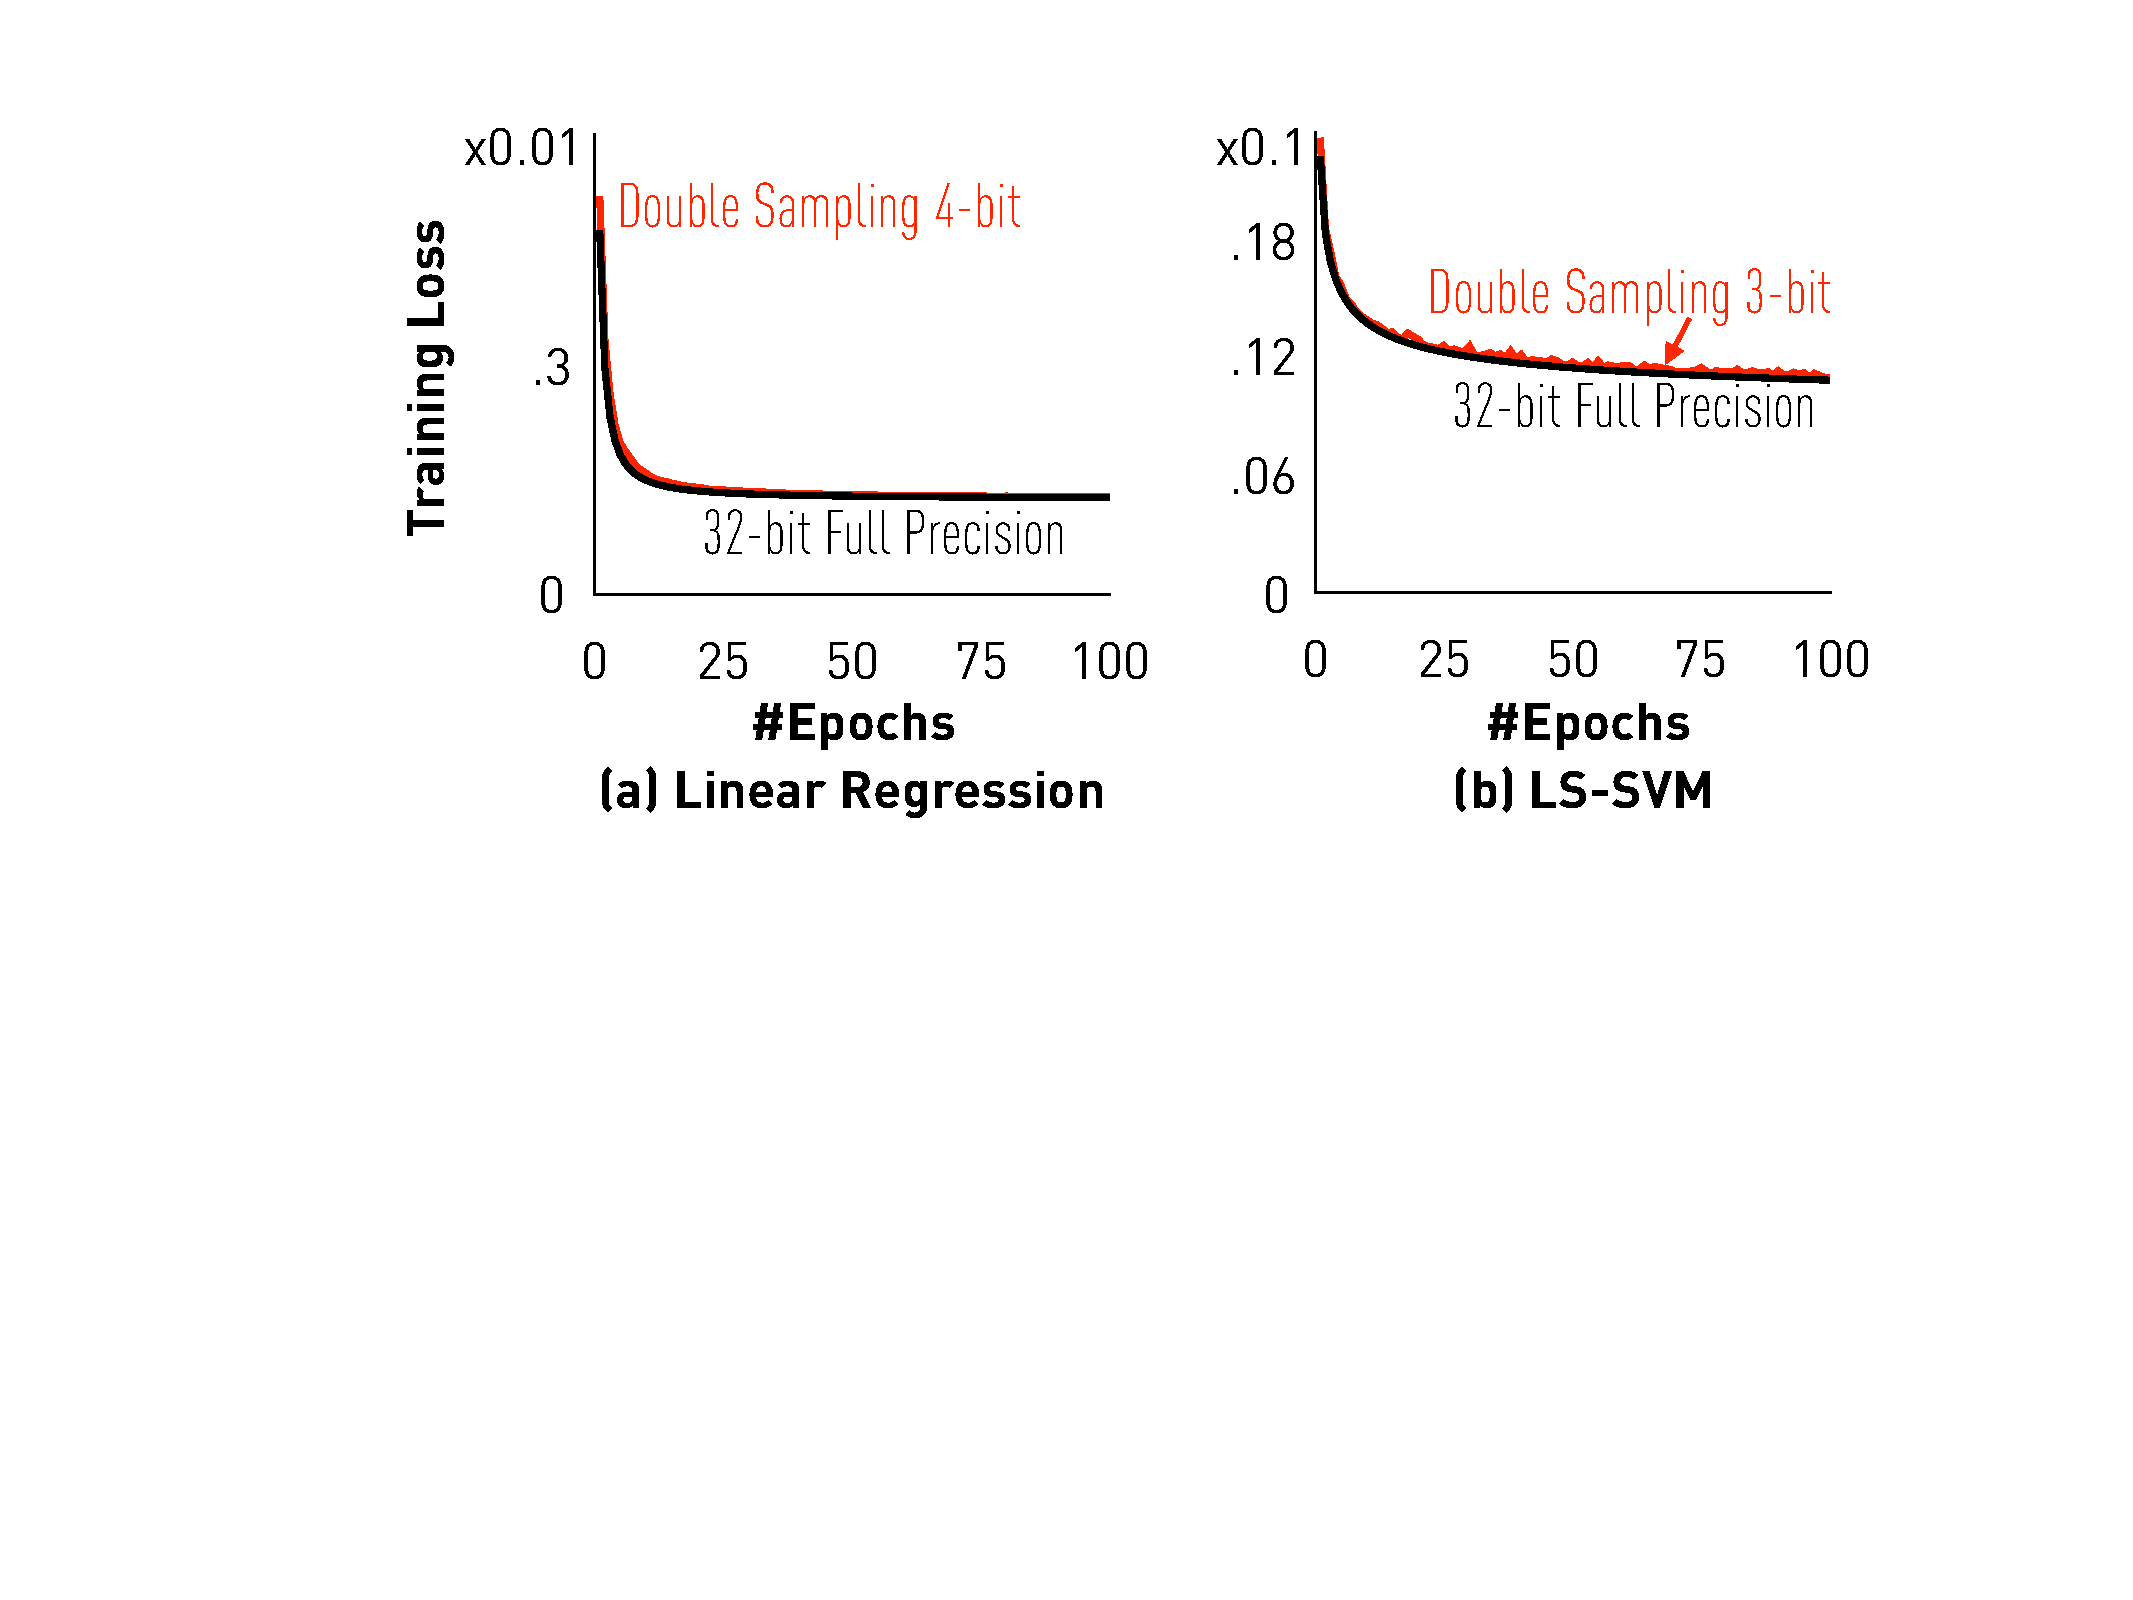
\includegraphics[width=0.68\columnwidth]{final-experiments/linearmodel} 
\vspace{-1em}
\caption{Linear models with end-to-end low precision.}
\vspace{-1.5em}
\label{fig:convergence}
\end{figure}

\vspace{-1em}
\subsection{Linear Models}
\vspace{-0.5em}

For linear models, we validate that (1) 
with double sampling, SGD with low
precision converges---in
comparable empirical 
convergence rates---to the same solution
as SGD with full precision; and
(2) implemented on FPGA, our low-precision
prototype achieves significant speedup
because of the decrease in bandwidth
consumption.

\vspace{-1.5em}
\paragraph{Convergence}

Figure~\ref{fig:convergence} illustrates
the result of training linear models:
(a) linear
regression and (b) least squares SVMs,
with end-to-end low-precision and 
full precision. For
low precision, we pick the 
smallest number of bits that
results in a smooth convergence
curve. We compare the final 
training loss in both settings 
and the convergence rate.

\vspace{-0.5em}
We see that, for both linear regression 
and least squares SVM,
using 3- or 4-bit is always enough
to converge to the same solution
with comparable convergence rate. 
This validates our prediction that
double-sampling provides an
unbiased estimator of the gradient.
Considering the size of input
samples that we need to read, we
could potentially save 8--10$\times$ 
memory bandwidth compared to using 
32-bit. 

\vspace{-1em}
\paragraph{Speedup}
We implemented our low-precision 
framework on a state-of-the-art 
FPGA platform. We leave the detailed 
implementation to the full version.
This implementation assumes the input
data is already quantized and
stored in memory (data can be
quantized during the
first epoch).

\vspace{-0.5em}
Figure~\ref{fig:speedup} illustrates 
the result of (1) our FPGA
implementation with quantized data,
(2) FPGA implementation with 32-bit
data, and (3) Hogwild! running with
10 CPU cores. 
Observe that all approaches
converge to the same solution.
FPGA with quantized data converges
6-7$\times$ faster
than FPGA with full precision
or Hogwild!. The FPGA implementation
with full precision is
memory-bandwidth bound, and by using our framework on quantized data, we save 
up to 8$\times$ memory-bandwidth, which
explains the speedup.


\begin{figure}[t]
\centering
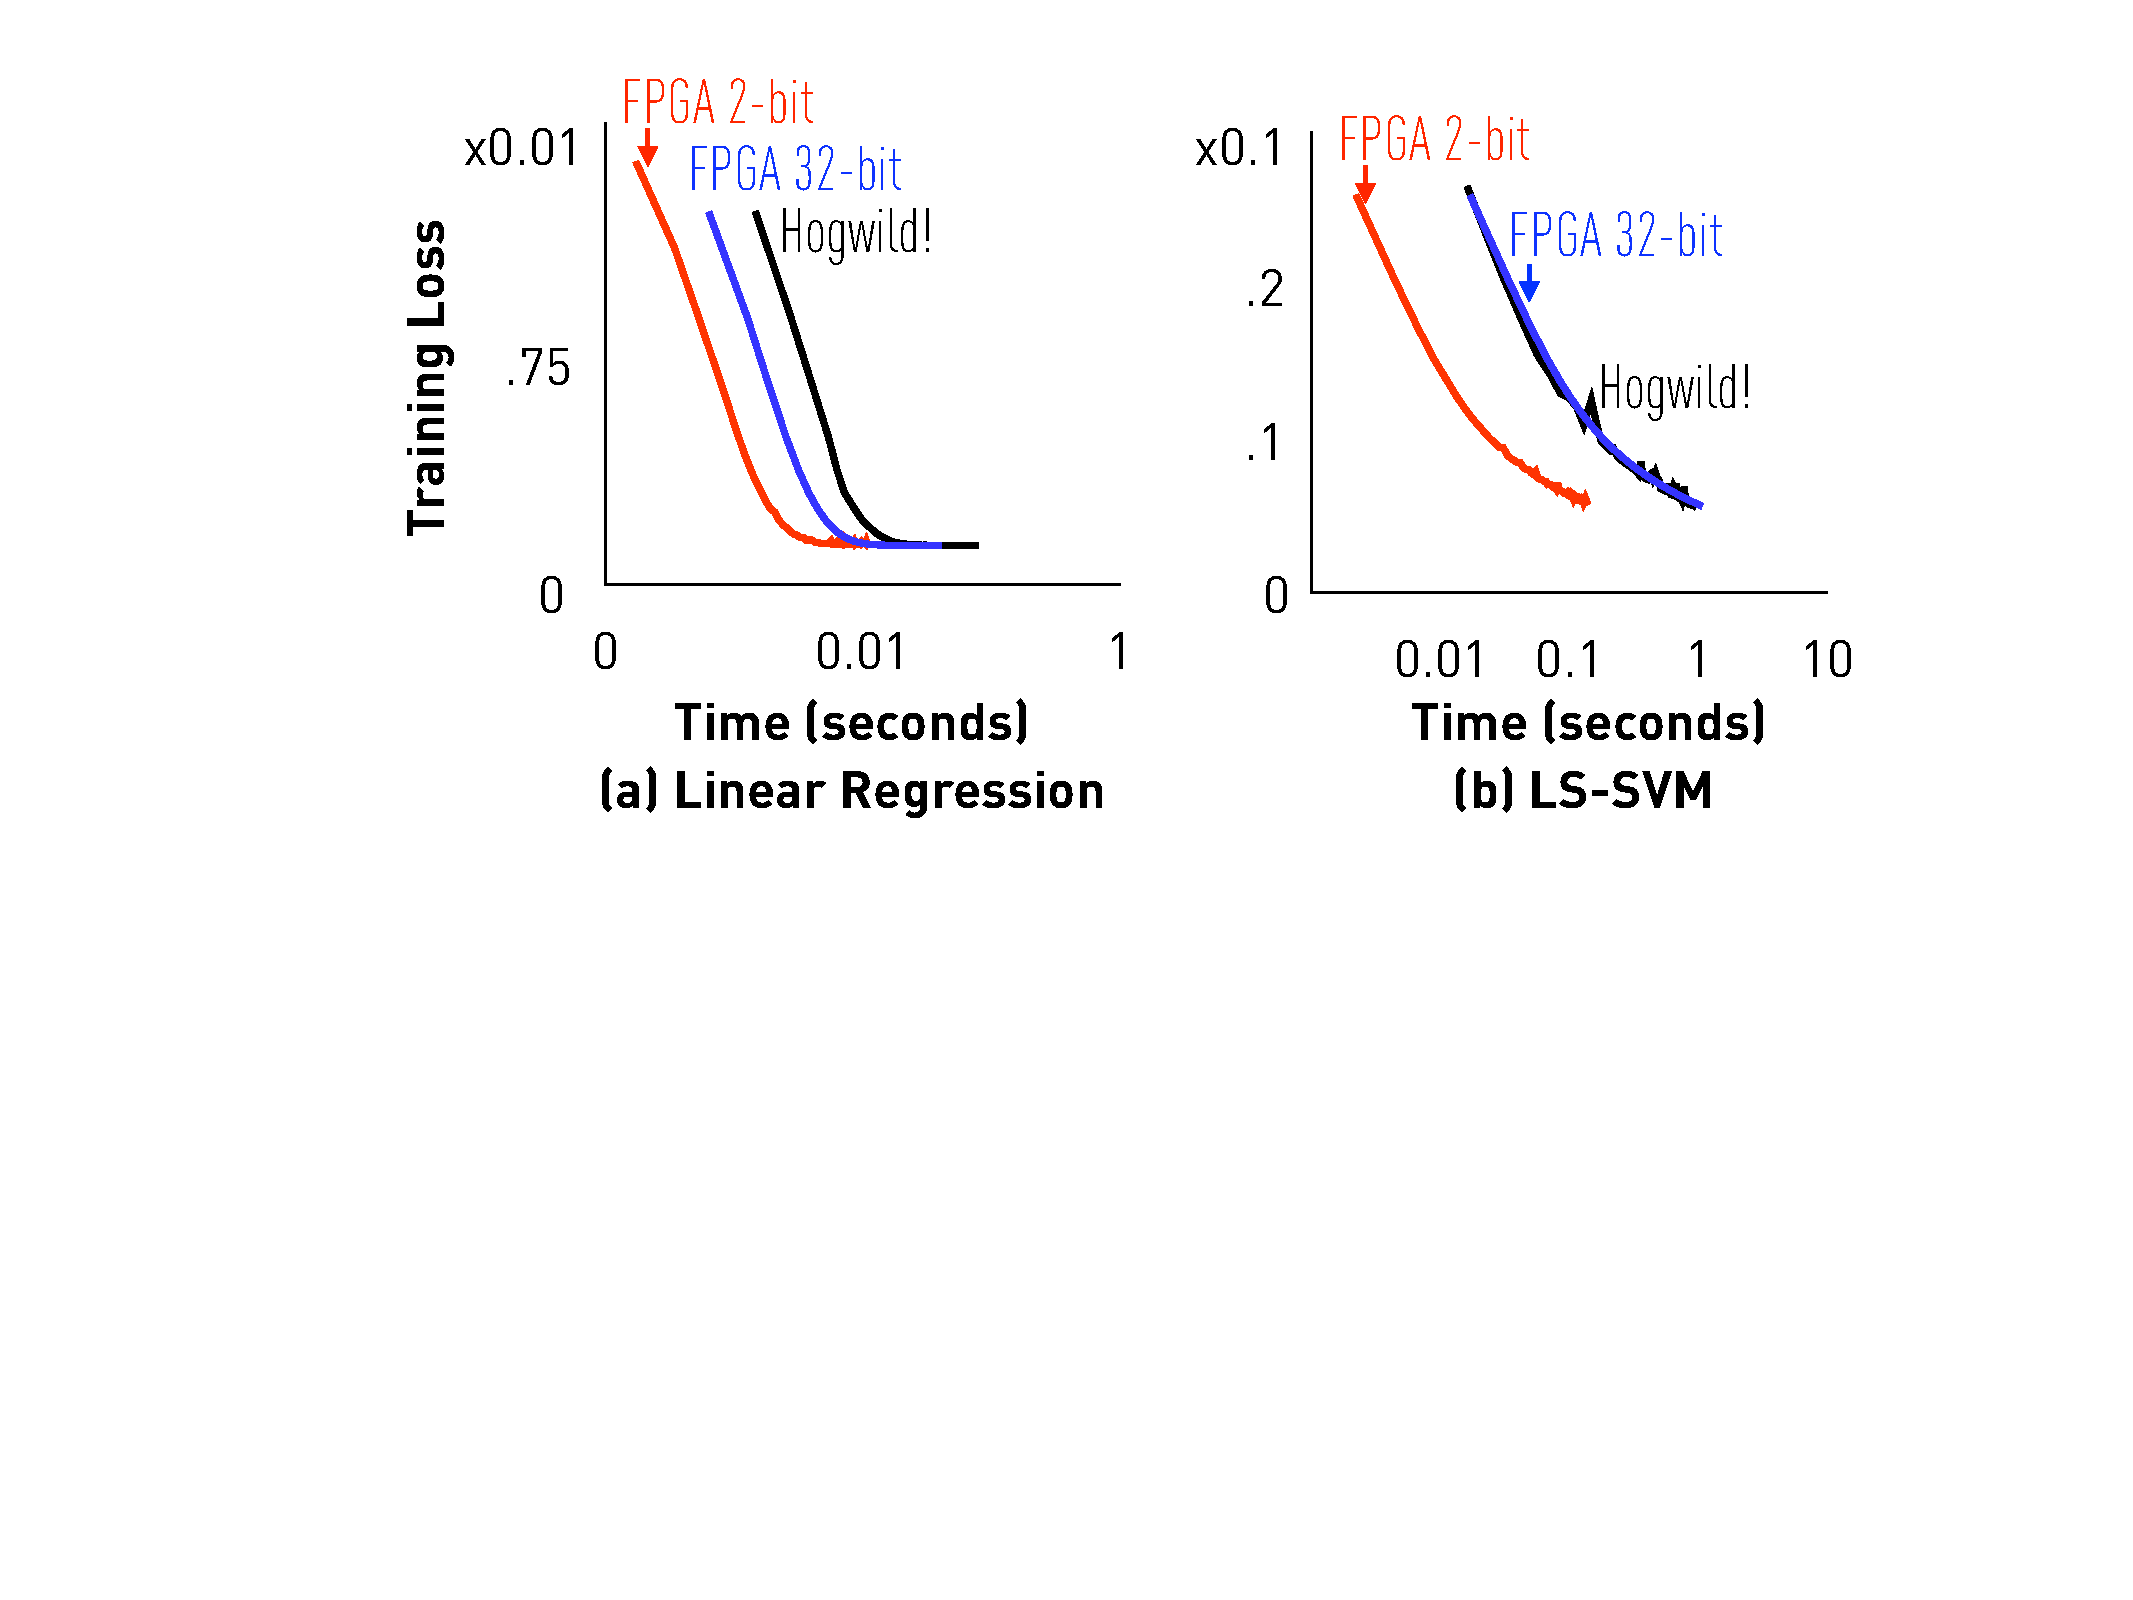
\includegraphics[width=0.68\columnwidth]{final-experiments/linear-fpga} 
\vspace{-1em}
\caption{FPGA implementation of linear models.}
\vspace{-2em}
\label{fig:speedup}
\end{figure}

\begin{figure}[t]
\centering
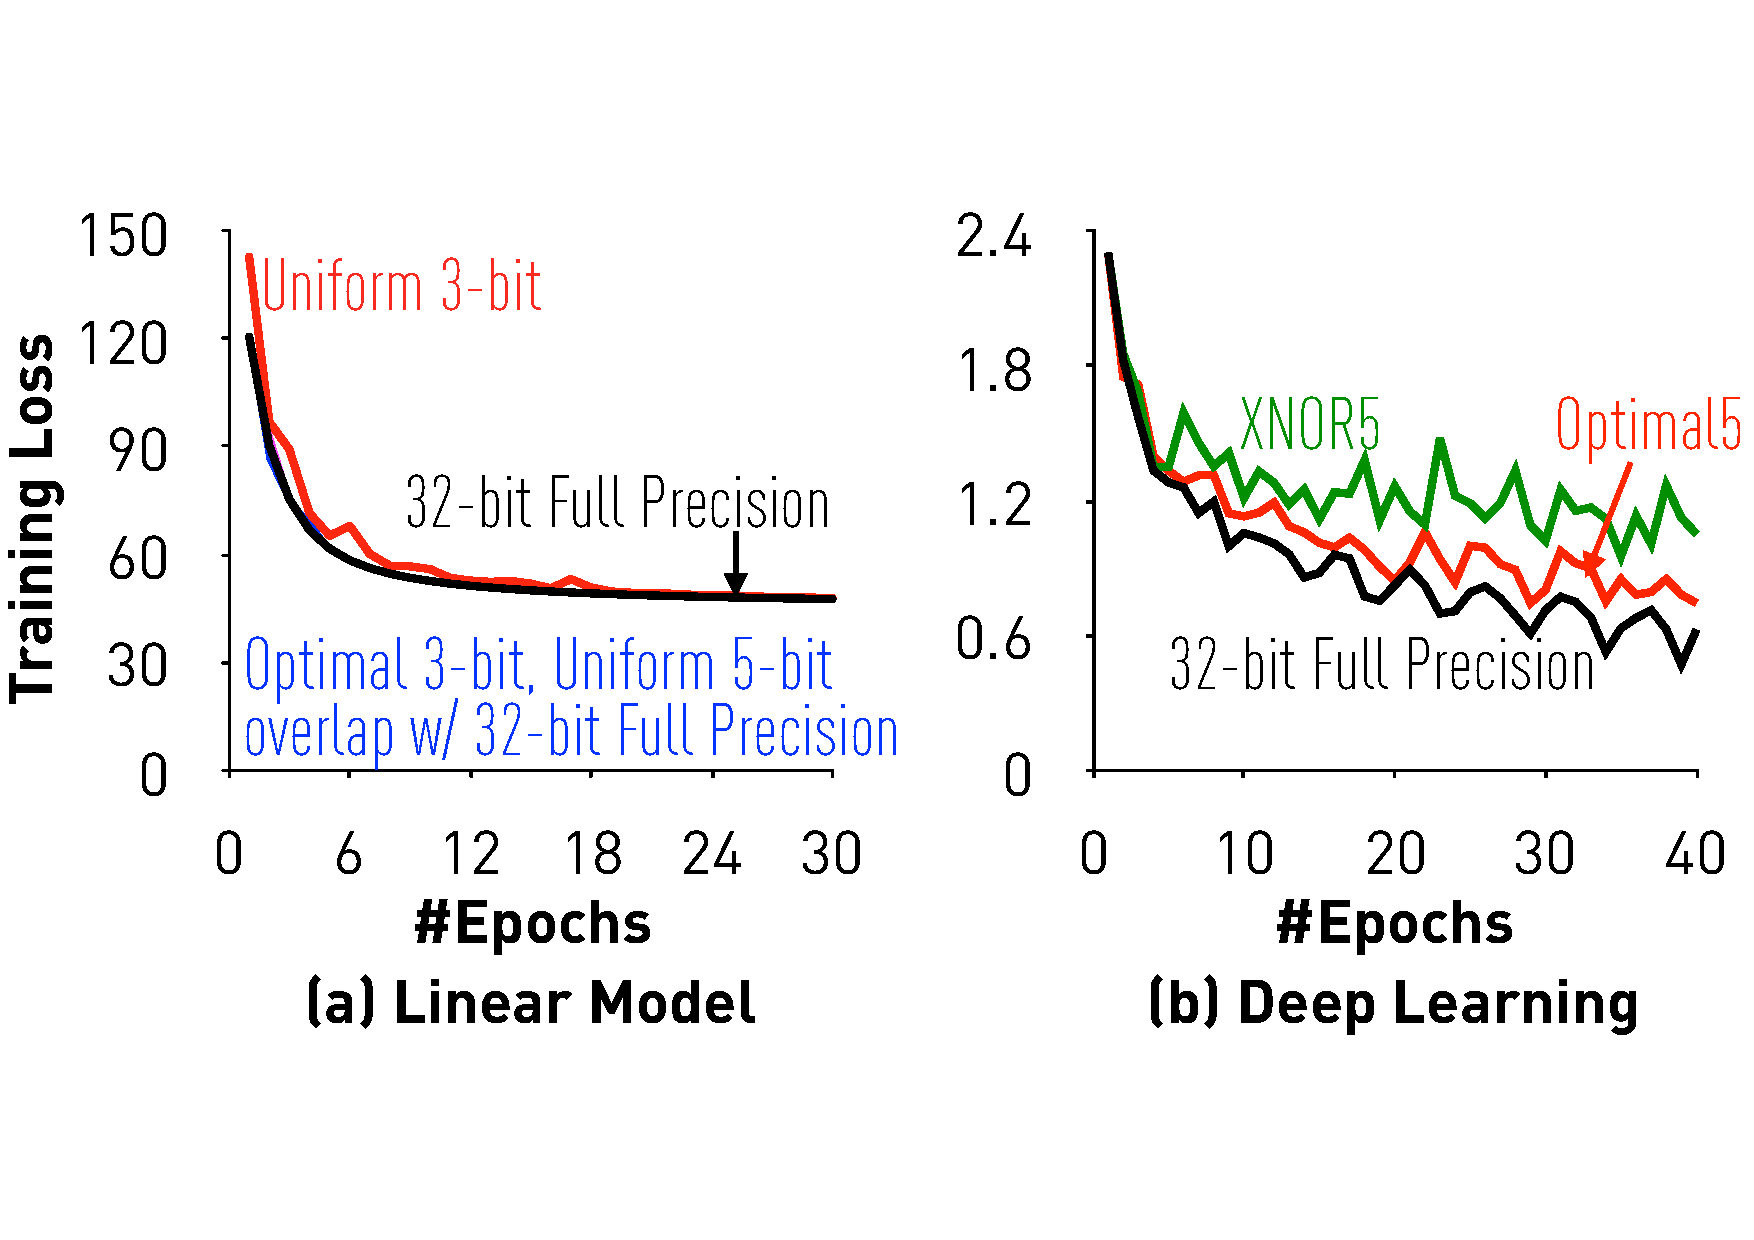
\includegraphics[width=0.68\columnwidth]{final-experiments/optimal} 
\vspace{-1em}
\caption{Optimal quantization strategy.}
\vspace{-2em}
\label{fig:optimal}
\end{figure}

\vspace{-1em}
\subsection{Data-Optimal Quantization Strategy}
\vspace{-0.5em}

We validate that, with our data-optimal quantization strategy, we can 
significantly decrease the number of 
bits that double-sampling requires to 
achieve the same convergence.
Figure~\ref{fig:optimal}(a) illustrates
the result of using 3-bit and 5-bit
for uniform quantization and optimal 
quantization on the {\bf YearPrediction}
dataset. We see that,
while uniform quantization needs 5-bit
to converge smoothly, optimal
quantization only needs 3-bit. 
We save almost $1.7\times$ number of 
bits by just allocating quantization points carefully.

\vspace{-1em}
\subsection{Extensions to Deep Learning}
\vspace{-0.5em}

We validate that our data-optimal quantization
strategy can be used in training deep neural
networks. We take Caffe's CIFAR-10 tutorial~\cite{Caffe:CIFAR10}
and compare three different quantization
strategies: (1) Full Precision, (2) XNOR5, 
a XNOR-Net implementation that, following
the multi-bits strategy in
the original paper, quantizes data into
five uniform levels, and (3)
Optimal5, our quantization strategy with
five optimal quantization levels. As
shown in Figure~\ref{fig:optimal}(b), Optimal5
converges to a significantly lower training 
loss compared with XNOR5. Also,
Optimal5 achieves $>$5 points higher testing accuracy over XNOR5.
This illustrates the improvement
obtainable by training a neural network with
a carefully chosen quantization strategy.



\begin{figure}[t]
\centering
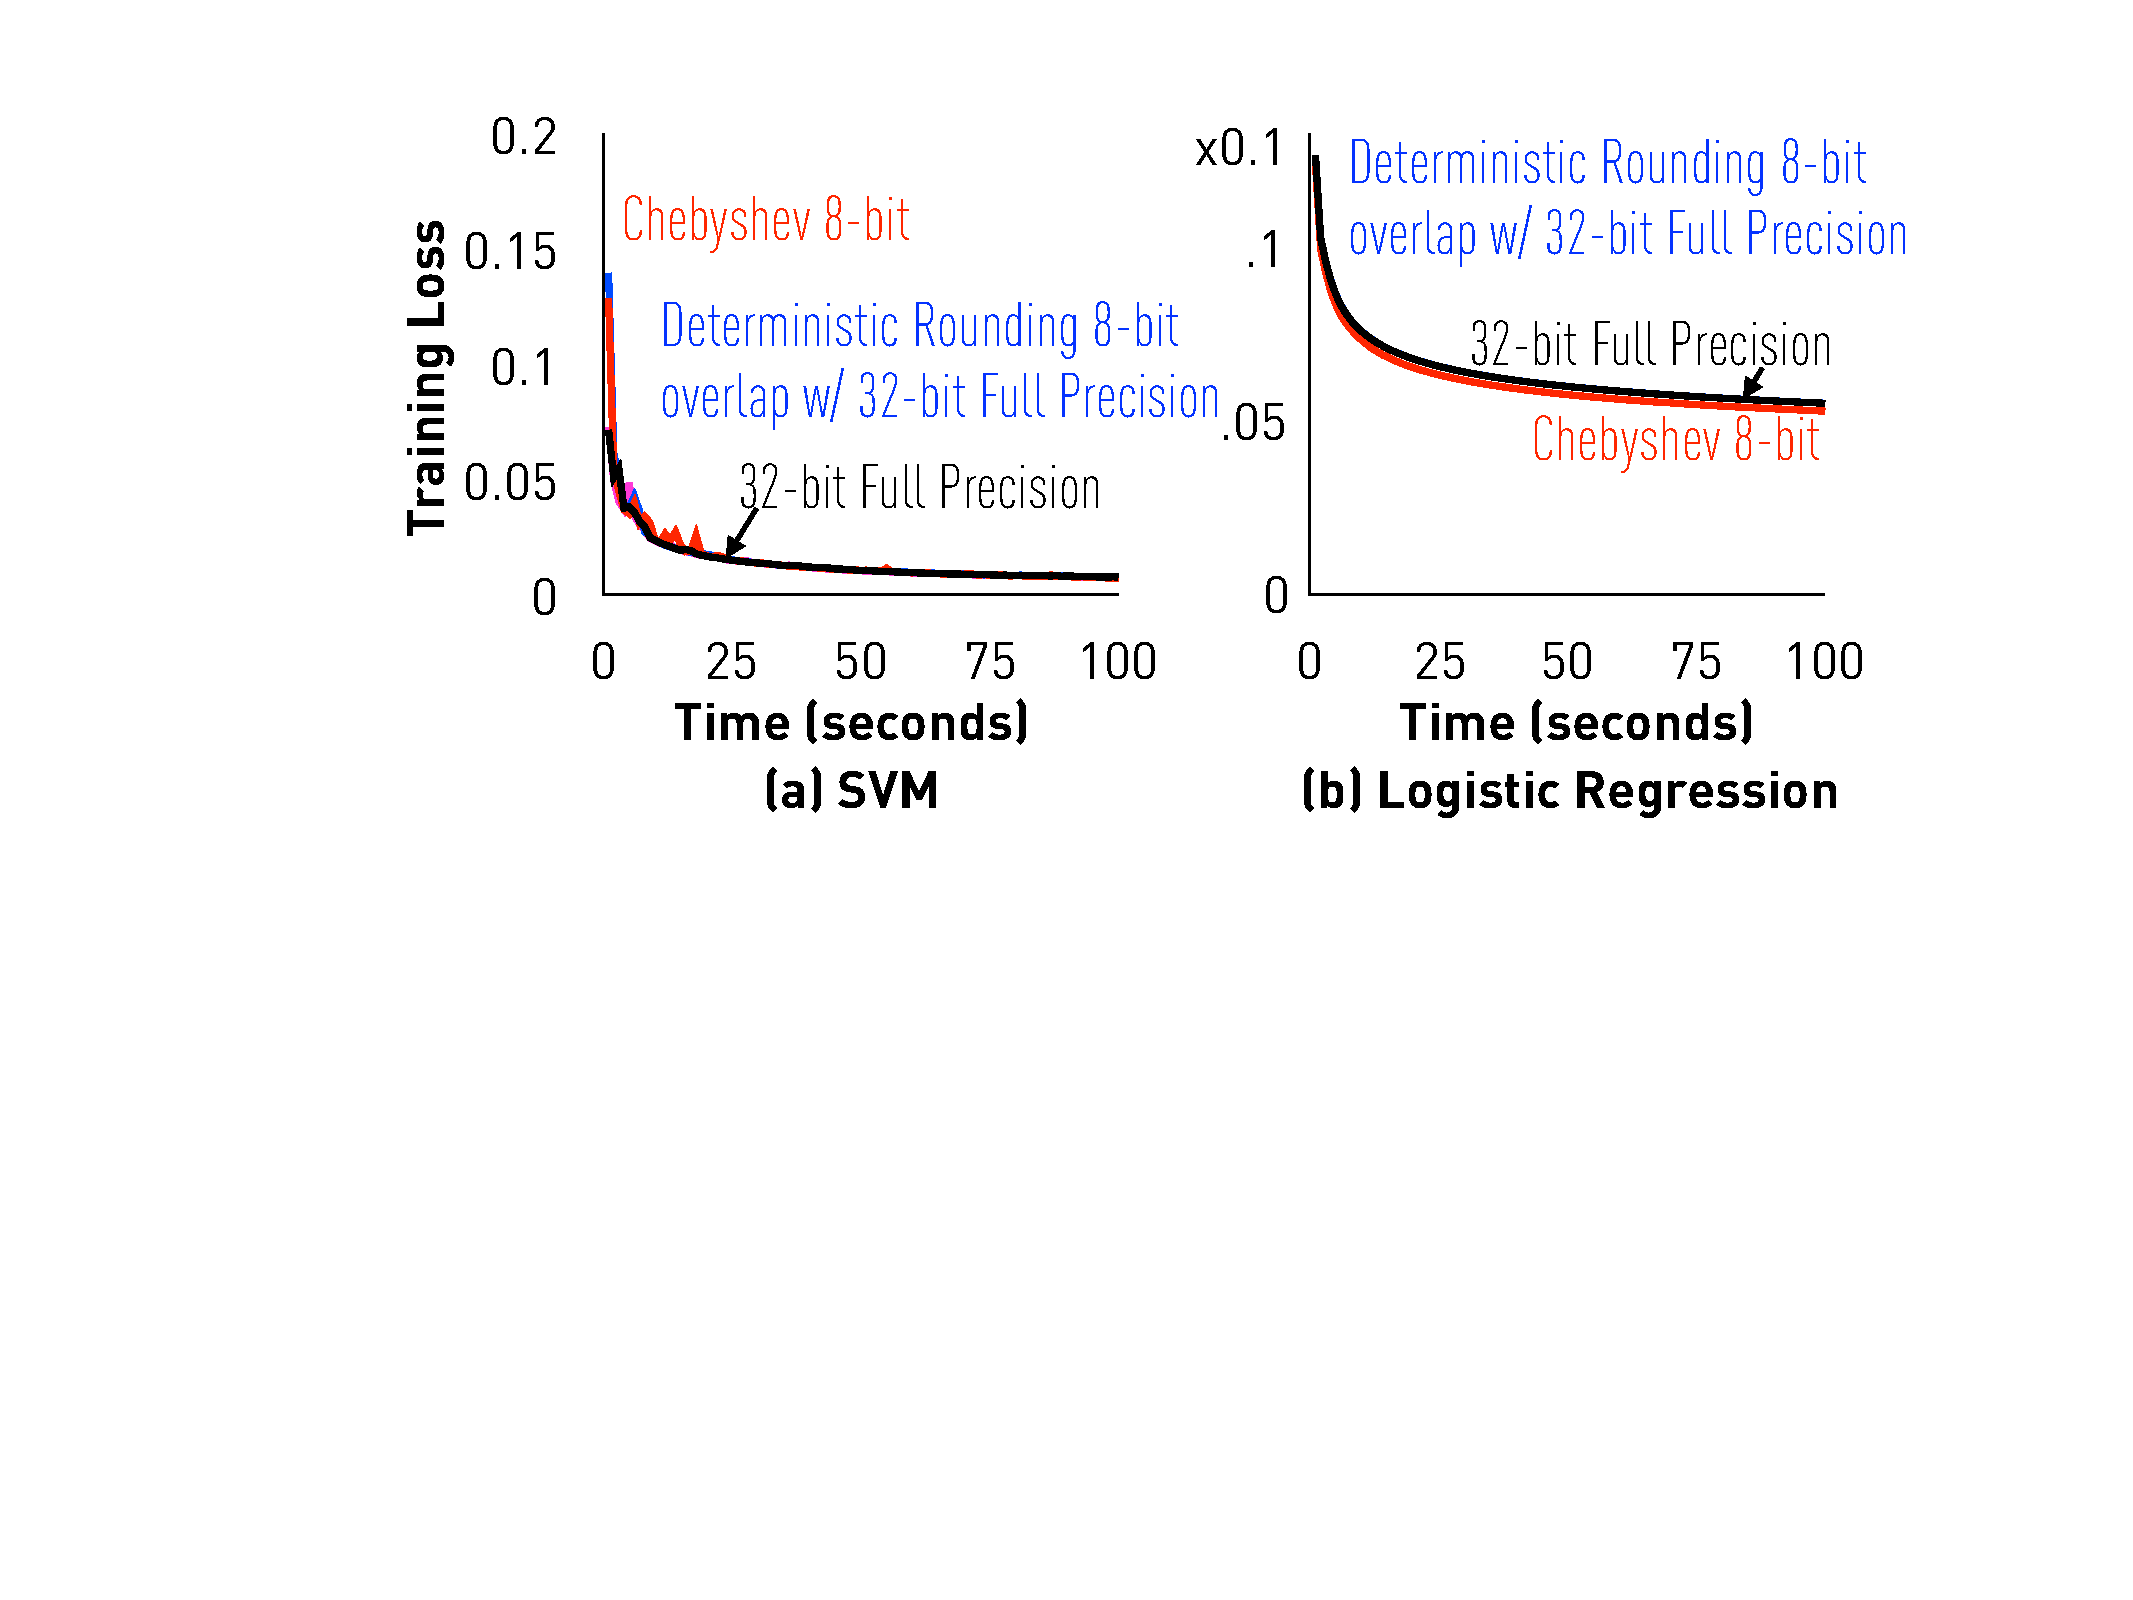
\includegraphics[width=0.68\columnwidth]{final-experiments/chebyshev} 
\vspace{-1.2em}
\caption{Non-linear models with Chebyshev approximation.}
\vspace{-1.9em}
\label{fig:chebyshev}
\end{figure}

\vspace{-1em}
\subsection{Non-Linear Models}
\vspace{-0.5em}

We validate that (1) our Chebyshev 
approximation approach is able to
converge to almost the same solution 
with 8-bit precision for both SVM
and logistic regression;
and (2) we are nevertheless able to construct
a straw man with 8-bit deterministic 
rounding or naive stochastic rounding
to achieve the same quality and convergence 
rate.

\vspace{-1.5em}
\paragraph{Chebyshev Approximations}

Figure~\ref{fig:chebyshev} illustrates
the result of training SVM
and logistic regression 
with Chebyshev approximation. Here,
we use Chebyshev polynomials up to
degree 15 (which requires 16 samples
that can be encoded with 4 extra 
bits). For each sample, the precision
is 4-bit, and therefore, in total
we use 8-bit for each single number
in input samples. We see that, 
with our quantization framework,
SGD converges to similar training loss 
with a comparable empirical convergence 
rate for both SVM and logistic regression.
We also experience no loss in test accuracy.



\vspace{-1.5em}
\paragraph{Negative Results}

We are able to construct the following,
much simpler strategy that also
uses 8-bit to achieve the same quality
and convergence rate as our
Chebyshev. In practice, as both
strategies incur bias on the result,
we do {\em not} see strong reasons to
use our Chebyshev approximation, thus
we view this as a negative result.
As shown in Figure~\ref{fig:chebyshev},
if we simply round the input samples
to the nearest 8-bit fix point
representation (or do rounding
stochastically), we achieve the
same, and sometimes better,
convergence than our Chebyshev 
approximation.

\vspace{-1em}
\section{Related Work} 
\vspace{-1em}

There has been significant work on ``low-precision SGD''~\cite{DeSa:NIPS:2015,Alistarh:2016:ArXiv}. 
These results provide
theoretical guarantees only for quantized gradients.
The model and input samples, on the other hand, are much more difficult
to analyze because of the non-linearity. We focus on {\em end-to-end}
quantization, for all components.

\vspace{-1em}
\paragraph{Low-Precision Deep Learning.}

Low-precision training of deep neural networks has been studied
intensively and many heuristics work well for a subset of networks.
OneBit SGD~\cite{Frank:2014:Interspeech} provides
a gradient compression heuristic developed in the context of deep 
neural networks for speech recognition. There are successful 
applications of end-to-end quantization to training neural networks that 
result in little to no quality loss~\cite{hubara2016quantized,
rastegari2016xnor,zhou2016dorefa,miyashita2016convolutional,li2016ternary,gupta2015deep}. They quantize weights, activations, and gradients 
to low precision (e.g., 1-bit) and revise the backpropagation 
algorithm to be aware of the quantization function.
The empirical success of this work inspired this paper, in which we try
to provide a {\em theoretical} understanding of end-to-end low-precision
training for machine learning models.
Another line of research concerns inference and model
compression of a pre-trained model~\cite{vanhoucke2011improving,gong2014compressing,Han:2016:ICLR,lin2016fixed,kim2016bitwise,kim2015compression,wu2016quantized}.
In this paper, we focus on training and leave the study of
inference for future work.

\vspace{-1.2em}
\paragraph{Low-Precision Linear Models.}

Quantization is a fundamental topic studied by the
DSP community, and there has been research on
linear regression models in the presence of quantization
error or other types of noise. For example,
\citet{Gopi:2013:ICML} studied compressive sensing
with binary quantized measurement, and a two-stage algorithm was proposed to recover the sparse high-precision solution up to a scale factor.
Also, the
classic errors-in-variable model~\cite{Hall:2008:Book}
could also be relevant if quantization is treated 
as a source of ``error.'' In this paper, we scope
ourselves to the context of stochastic gradient descent, 
and our insights go beyond simple linear models.
For SVM the straw man approach 
can also be seen as a very simple case of kernel 
approximation~\cite{Cortes:2010:AISTATS}.

\vspace{-1.2em}
\paragraph{Other Related Work.} Precision of data
representation is a key design decision
for configurable hardwares such as FPGA. There have been attempts to
lower the precision when training on such hardware~\cite{Kim:2011:ICASSP}. 
These results are mostly empirical; we
aim at providing a theoretical understanding, which 
enables new algorithms.

\vspace{-1.5em}
\section{Discussion}
\label{sec:conclusions}

\vspace{-1em}
Our motivating question was whether end-to-end low-precision data representation can enable efficient computation with convergence guarantees. 
We show that a relatively simple stochastic quantization framework can achieve this for linear models. 
With this setting, as little as two bits per model dimension are sufficient for good accuracy, and can enable a fast FPGA implementation.  

\vspace{-0.5em}
For non-linear models, the picture is more nuanced. 
In particular, we find that our framework can be generalized to this setting, and that in practice \emph{8-bit is sufficient} to achieve good accuracy on a variety of tasks, such as SVM and logistic regression. 
However, in this generalized setting, naive rounding has similar performance on many practical tasks. 

\vspace{-0.5em}
It is interesting to consider the rationale behind these results. Our framework is based on the idea of \emph{unbiased approximation} of the original SGD process. For linear models, this is easy to achieve. For non-linear models, this is harder, and we focus on guaranteeing arbitrarily low bias. 
However, for a variety of interesting functions such as hinge loss, guaranteeing low bias requires complex approximations. In turn, these increase the variance. The complexity of the approximation and the resulting variance increase force us to increase the \emph{density} of the quantization, in order to achieve good approximation guarantees. 


\cleardoublepage





\bibliographystyle{icml2017}
\bibliography{low-precision.bib}


\end{document}